% for sublime text 3
%!TEX root = diss.tex

\chapter{Related Work}
\label{ch:rel-work}
 
The task of coherence modeling has received a lot of attention due to its key impact in other natural language processing systems. 
In this thesis, we propose a novel approach to local coherence modeling based on graph representations of texts. 
We apply our approach to two types of graphs.  
The first type captures coreferent relations between named entity mentions in a text.
The second one represents lexical relations among words in a text.  
Our coherence model is evaluated with respect to its impact on readability assessment and text summarization. 

Accordingly, we first review entity-based approaches to local coherence (Section \ref{sec:rel-entity-models}). 
We then survey lexical approaches (Section \ref{sec:rel-ent-grid}). 
Finally, we discuss applications for local coherence model that have been introduced in the literature, particularly readability assessment and summarization tasks (Section \ref{sec:rel-coh-applications}). 
% A coherent text consists of a sequence of topics in a structured way \cite{marcu97b,hearst97,gallery03}. 
% Related models are often constructed as sequential topical models. 
% Topics are modeled by a language model \cite{blei01} or Bayesian topic models \cite{eisenstein08}.
% For modeling the temporal structure, early research uses a Hidden Markov Model \cite{barzilay04}, and  
% later research employs sequential neural networks \cite{}. 

\section{Entity-Based Approaches to Local Coherence}
\label{sec:rel-entity-models}

The primary steps of the research presented in this thesis are inspired by entity-based models. 
In this section, we explain details of two popular entity-based coherence models: the entity grid model, and the entity graph model. 
We also briefly discuss their extensions.  

\paragraph{Historical Review.} Entity-based approaches to local coherence have a long history within the linguistic literature \cite{kuno72,halliday76,prince81a,joshi98}.
Most approaches are common in the primary assumption that coherence is perceived with respect to how entities are introduced and discussed in a text. 
Texts that keep referring to similar entities are supposed to be more coherent than those with random and unexpected switches from one entity to another. 
This premise is supported by different theories, one of which is Centering Theory \cite{grosz95,joshi98} (see Chapter \ref{ch:coherence}). 

A great deal of research has been devoted to directly implement Centering Theory \cite{miltsakaki00,karamanis04a}. 
This is challenging because a computational model needs to determine how to instantiate parameters of the theory that are often underspecified. 
Interestingly, \newcite{poesio04b} note that even for basic parameters of Centering Theory such as ``utterance'', ``realization'', and ``ranking'' (see Chapter \ref{ch:coherence} for their definitions), multiple interpretations have been developed, because in the original theory of centering these concepts are not explicitly specified. 
As an instance, in some papers entities are ranked with respect to the grammatical function \cite{brennan87,grosz95} of entity occurrences in a text, and in some other papers those are ranked with respect to the position of entity mentions in sentences \cite{prince81a}, the familiarity status, or the thematic role \cite{strube.cl99,moens08}.
As a result, two instantiations of the same theory make different predictions for the same input.  

Some studies try to avoid this by finding an instantiation of parameters which is most consistent with observable data \cite{strube.cl99,karamanis04a,poesio04b}. 
Some others adopt a specific instantiation so that the performance of the coherence model improves for a specific task. 
For example, \newcite{miltsakaki00} annotate a corpus of student essays with entity transition information, and then show that the distribution of transitions correlates with human grades. 
Analogously, \newcite{hasler03} investigate whether the centering theory can be used in evaluating the readability of text by annotating summaries produced by humans or machines with the entity transition information. 
To sum up, \newcite{poesio04b} demonstrate that the predictive power of the models that directly implement centering theory is highly sensitive to their parameter instantiations.  

\newcite{barzilay05a,barzilay08} propose a general framework for coherence modeling.  
The main goal of this framework is to eliminate the need to human annotations for parameters in the centering theory, regardless of what the evaluation task is. 
By some inspirations from the theory, this model hypothesizes that the distribution of entities in coherent texts reveal certain regularities that make these texts recognizable from incoherent ones. 
These regularities can be learned by machine learning approaches.  
Since this model has been the core of many research in the area of coherence modeling (including the research presented in this thesis), we explain details of this model.    

\subsection{The Entity Grid Model}
\label{sec:rel-ent-grid} 

\newcite{barzilay05a,barzilay08} are the first researchers who proposed a general  computational approach to local coherence modeling based on the entity relations across adjacent sentences.  
Supported by some linguistic work such as Centering Theory \cite{grosz95} and other entity-based theories of discourse \cite{prince81a}, they assume that the distribution of entities in coherent texts exhibits certain regularities that can be reflected in a grid topology, which is called the entity grid. 
In this thesis we refer to this model as the \emph{entity grid} model, because its key idea is to represent the distribution of entities (see Chapter \ref{ch:coherence} for definition of entities) across sentences in a text by a grid.   
In practice, mentions of an entity are linked together in order to show that they are referring to the same entity. 
Connections between mentions not only show that those are referring to the same entity, but also indicate that sentences that contain those mentions are (almost) about the same topic or information \cite{barzilay08}. 

\subsubsection{Text Representation: Entity Grid}

In this model each text is represented by a grid, which is a two dimensional array whose rows correspond to entities, and columns are matching to sentences.
An entry $r_{i;j}$ in a grid describes the syntactic role of entity $i$ in sentence $j$ if the entity is mentioned in the sentence. 
The syntactic roles are categorized as subject (S), object (O), or all other syntactic roles (X). 
In addition, if an entity is not mentioned in a sentence, a special marker (-) fills the corresponding entry $r_{i;j}$. 
Finally, if a sentence contains several mentions of one entity, their corresponding entry describes the most important grammatical role of the mentions: subject if possible, then object, or finally other. 

The discussion of the grid develops around the important question of which textual units are to be considered mentions of an entities, and how different mentions are to be linked to represent an entity. 
A perfect solution in this regard would use coreference resolution to recognize mentions, noun phrases, and link arbitrary mentions to the same entities and discarding noun phrases which do not correspond to an entity. 
Since coreference resolution systems are far from prefect\footnote{The highest reported precision of a coreference system on the ? dataset is ?.}, and tend to work even more poorly on incoherent texts, this approach is not generally one utilized.  
Moreover, a non-perfect general coreference system introduces more noise to a coherence model than what it fixes \cite{barzilay08}.  
As an alternative, implementations of the entity grid model tend to employ all noun phrases as mentions and perform a heuristic, but strict and simple, coreference resolution. 
They connect all mentions that have an identical head noun as one entity. 
Detailed discussions of this heuristic are given in \newcite{poesio04c} and \newcite{elsner10}. 

As an example consider the sample text\footnote{The text with ID D31010, taken from Document Understanding Conference (DUC-?) dataset, which we use in one of our experiments. Numbers are not marked because they are filtered out in preprocessing.} in Example \ref{ex:rel-text}. 
In this example, noun phrases are marked with brackets as an indication of mentions. 
Mentions in a sentence are associated with their syntactic functions in the sentence, noted with a letter (S: subject, O: object, and X: others) next to the brackets. 
%/hits/fast/nlp/mesgarmn/Data/ACL13/SummaryCoherence/texts/
%D31010.M.100.T.E.txt. Nubembers (e.g. 29) are filtered out in preprocessing.}  

\begin{examples}
\label{ex:rel-text}
\begin{tabular}{l@{\space}p{12.5cm}}
 $s_0$: &[An arctic cold wave]\textbf{\textsubscript{S}}, [the worst]\textbf{\textsubscript{X}} in [10 years]\textbf{\textsubscript{X}}, hit [parts]\textbf{\textsubscript{O}} of [Europe]\textbf{\textsubscript{X}}, bringing [sub-zero temperatures]\textbf{\textsubscript{O}} and killing [scores]\textbf{\textsubscript{O}} of [people]\textbf{\textsubscript{X}}. \\

 $s_1$: & Hardest hit were [Poland]\textbf{\textsubscript{S}}, [Bulgaria]\textbf{\textsubscript{S}}, and [Romania]\textbf{\textsubscript{S}} as well as [parts]\textbf{\textsubscript{S}} of [central]\textbf{\textsubscript{X}} and [eastern France]\textbf{\textsubscript{X}}. \\

$s_2$: &In [Poland]\textbf{\textsubscript{X}}, [three weeks]\textbf{\textsubscript{X}} of [sub-zero temperatures]\textbf{\textsubscript{X}} killed [at least 85 people]\textbf{\textsubscript{O}} in [November]\textbf{\textsubscript{X}}, 29 more than in [all]\textbf{\textsubscript{X}} of [the previous winter]\textbf{\textsubscript{S}}. \\


$s_3$: &[Most]\textbf{\textsubscript{S}} of [the victims]\textbf{\textsubscript{X}} were homeless [whose deaths]\textbf{\textsubscript{X}} by [exposure]\textbf{\textsubscript{X}} were alcohol related. \\

$s_4$: &[Blizzards]\textbf{\textsubscript{X}} and [cold temperatures]\textbf{\textsubscript{S}} also hit [Bulgaria]\textbf{\textsubscript{X}} and [Romania]\textbf{\textsubscript{O}}, stranding [hundreds]\textbf{\textsubscript{O}} in [their cars]\textbf{\textsubscript{X}}. \\

$s_5$: &Elsewhere, [snow]\textbf{\textsubscript{S}} blanketed [the Italian island]\textbf{\textsubscript{O}} of [Capri]\textbf{\textsubscript{X}} for [the first time]\textbf{\textsubscript{X}} in [10 years]\textbf{\textsubscript{X}}. 
\end{tabular}
\end{examples}
%%(ROOT (S (NP (NP (DT An) (JJ arctic) (JJ cold) (NN wave)) (, ,) (NP (NP (DT the) (JJS worst)) (PP (IN in) (NP (CD 10) (NNS years)))) (, ,)) (VP (VBD hit) (NP (NP (NNS parts)) (PP (IN of) (NP (NNP Europe)))) (, ,) (S (VP (VP (VBG bringing) (NP (JJ sub-zero) (NNS temperatures))) (CC and) (VP (VBG killing) (NP (NP (NNS scores)) (PP (IN of) (NP (NNS people)))))))) (. .)))

%%(ROOT (S (S (VP (ADVP (RBS Hardest)) (VBN hit))) (VP (VBD were) (NP (NP (NP (NNP Poland)) (, ,) (NP (NNP Bulgaria)) (, ,) (CC and) (NP (NNP Romania))) (CONJP (RB as) (RB well) (IN as)) (NP (NP (NNS parts)) (PP (IN of) (NP (NP (JJ central)) (CC and) (NP (JJ eastern) (NNP France))))))) (. .)))

%%(ROOT (S (PP (IN In) (NP (NNP Poland))) (, ,) (NP (NP (CD three) (NNS weeks)) (PP (IN of) (NP (JJ sub-zero) (NNS temperatures)))) (VP (VBD killed) (NP (QP (IN at) (JJS least) (CD 85)) (NNS people)) (PP (IN in) (NP (NNP November))) (, ,) (PP (ADVP (NP (CD 29)) (RBR more)) (IN than) (IN in) (NP (NP (DT all)) (PP (IN of) (NP (DT the) (JJ previous) (NN winter)))))) (. .)))

%%(ROOT (S (NP (NP (JJS Most)) (PP (IN of) (NP (DT the) (NNS victims)))) (VP (VBD were) (ADJP (JJ homeless) (SBAR (WHNP (NP (WP$ whose) (NNS deaths)) (PP (IN by) (NP (NN exposure)))) (S (VP (VBD were) (ADJP (RB alcohol) (VBN related))))))) (. .)))

%%(ROOT (S (NP (NP (NNS Blizzards)) (CC and) (NP (JJ cold) (NNS temperatures))) (ADVP (RB also)) (VP (VBD hit) (NP (NNP Bulgaria) (CC and) (NNP Romania)) (, ,) (S (VP (VBG stranding) (NP (NNS hundreds)) (PP (IN in) (NP (PRP$ their) (NNS cars)))))) (. .)))

%%(ROOT (S (ADVP (RB Elsewhere)) (, ,) (NP (NN snow)) (VP (VBD blanketed) (NP (NP (DT the) (JJ Italian) (NN island)) (PP (IN of) (NP (NNP Capri)))) (PP (IN for) (NP (NP (DT the) (JJ first) (NN time)) (PP (IN in) (NP (CD 10) (NNS years)))))) (. .)))
%%

The corresponding entity grid for the text that is shown in Example \ref{ex:rel-text} is presented in Table \ref{tab:rel-egrid}. 
In this grid we follow \newcite{barzilay05a, barzilay08} and consider head nouns of noun phrases to represent the named entities that they are referring to. 
The coreferent mentions are detected by string match over head nouns. 

\begin{table}[!ht]	
	\begin{center}
		\begin{tabular}{lcccccc}
			\hline
			WAVE 			& S & - & - & - & - & - \\
			WORST 			& X & - & - & - & - & - \\
			YEARS 			& X & - & - & - & - & X \\
			PARTS 			& O & O & - & - & - & - \\
			EUROPE  		& X & - & - & - & - & - \\
			TEMPERATURES  	& O & - & X & - & S & - \\
			SCORES  		& O & - & - & - & - & - \\
			PEOPLE  		& X & - & O & - & - & - \\
			POLAND 			& - & O & X & - & - & - \\
			BULGARIA  		& - & X & - & - & - & - \\
			ROMANIA  		& - & X & - & - & O & - \\
			CENTRAL  		& - & X & - & - & - & - \\
			FRANCE  		& - & X & - & - & - & - \\
			NOVEMBER  		& - & - & X & - & - & - \\
			WEEKS 			& - & - & S & - & - & - \\
			ALL 			& - & - & X & - & - & - \\
			WINTER  		& - & - & X & - & - & - \\
			MOST 			& - & - & - & S & - & - \\
			VICTIMS  		& - & - & - & X & - & - \\
			DEATHS 			& - & - & - & X & - & - \\
			EXPOSURE  		& - & - & - & X & - & - \\
			BLIZZARDS  		& - & - & - & - & S & - \\
			HUNDREDS  		& - & - & - & - & O & - \\
			CARS  			& - & - & - & - & X & - \\
			TIME  			& - & - & - & - & - & X \\
			SNOW  			& - & - & - & - & - & S \\
			ISLAND 			& - & - & - & - & - & O \\
			CAPRI 			& - & - & - & - & - & X \\
			\hline
		\end{tabular}
		\caption{The entity grid representation of the text presented in Example \ref{ex:rel-text}. The rows represent entities and columns encode sentences. 
		If an entity is mentioned in a sentence, their corresponding entry in the gird indicates the grammatical role of the mention in the sentence, otherwise the entry is marked by ``--''.} 
		\label{tab:rel-egrid}
	\end{center}
\end{table}

It is worth noting that although entities in the original version of the entity grid are indicated by the head of a noun phrase (such as \emph{flight} in Example \ref{ex:rel-text}), \newcite{elsner11a} show that adding non-head nouns (like "the personal \textbf{country} flight" in Example \ref{ex:rel-text}) to a grid is beneficial to improve the representation power of the entity grid model. 
This enables the model to involve both head nouns and pre-modifiers in noun phrases to link sentences. 
Therefore, \newcite{elsner11a} consider all nouns (both \emph{country},\emph{flight} in the above example) in their entity grid representation.  
The non-head mentions are given the role X. 

\subsection{Pattern Definition: Grammatical Transitions}
%
The key hypothesis in the entity grid model is that the way that entities are distributed and that grammatical roles of entity occurrences change through a text reveal similar patterns in coherent texts.  
\newcite{barzilay05a,barzilay08} predefine all possible transitions that may occur for an entity in a text. 

More concretely, they define a transition pattern as a sequence of employed symbols with size $n$, $\{ S,O,X,\textit{--} \}^n$. 
Each pattern represents both entity occurrences between sentences, and the way that their syntactic roles in $n$ adjacent sentences are changing. 
For instance, for two adjacent sentences ($n=2$) there are $16$ possible patterns, which are shown in Table \ref{table:rel-egrid-pattern}.

\begin{table}[!ht]
	\begin{center}
		\resizebox{\columnwidth}{!}
		{%
			\begin{tabular}{@{}cccccccccccccccc@{}}
			\hline
			S S & S O & S X & S -- & 
			O S & O O & O X & O -- & 
			X S & X O & X X & X -- & 
			-- S & -- O & -- X & -- -- 
			\\\hline
			\end{tabular}
		}%
	\end{center}
	\caption{Patterns that are defined in the entity grid model.  
	They represent all possible entity occurrences in two adjacent sentences. 
	Symbols S (subject), O (object), and X (other) show grammatical role of an entity in a sentence. Symbol ``--'' encodes that an entity is not mentioned in a sentence.}
	\label{table:rel-egrid-pattern}
\end{table}

Each pattern that is shown in Table \ref{table:rel-egrid-pattern} represents one possible way that an entity may occur in two adjacent sentences. 
For example, pattern ``S O'' encodes that an entity appears in two adjacent sentences, and its syntactic role is changing from subject to object in sentences. 
As another example, consider pattern ``S --''. 
It indicates that an entity is referred to by a mention in the subject position of a sentence, but the entity has no mention in the immediately next sentence. 

\subsubsection{Coherence Representation: Probabilities of Transitions}
%
The entity grid model revolves around this assumption that coherent texts reveal certain regularities over the frequency of transitions or patterns \cite{barzilay05a,barzilay08}.    
The frequency of patterns can be used as an indicator to the preference of coherent texts in using or avoiding certain transitions. 
However, in order to prevent the model to be biased towards the text length, a probability for each pattern is computed, rather than the frequency. 	 
More formally, given the entity grid representation of a text, the probability of occurring a transition pattern in the grid is computed as follows:

\begin{equation}
p(t) = \frac{n(t)}{n(t^*)},
\end{equation}
where $t$ is a transition, $n(t)$ indicates the number of times that transition $t$ is occurring in the entity grid, and denominator $n(t^*)$ depicts the number of occurrences of all patterns whose length is as same as the length of $t$ in the grid. 
For instance consider the grid in Table \ref{tab:rel-egrid}, the probability of pattern ``O O'' is .01, which is computed as a ratio of its frequency, i.e. one, divided by the total number of patterns of length two, i.e., 140. 

\textbf{CHECK IF THIS GRID MATCHES WITH WHAT CAMILE GAVE YOU. IF NOT, YOU SHOULD SAY THAT THIS GRID, INCLUDING SYNTACTIC ROLES AND HEAD NOUN FINDERS, IS GENERATED BY BROWNCOHERENCE TOOLKIT. 
HOW IS IT POSSIBLE THAT A SENTENCE DOES NOT HAVE ANY SUBJECT, SEE S2}   

Each text can thus be viewed as a distribution defined over patterns. 
Therefore, the entity grid model represent the coherence property of a text by a fixed set of pattern sequences using a standard feature vector notation, where each feature is the probability of its corresponding pattern in the grid representation of the text.  
Table \ref{tab:rel-egrid-probs} shows the feature vector representation of the gird presented in Table \ref{tab:rel-egrid} using all transitions of length two. 

\begin{table}
	\begin{center}
		\resizebox{\columnwidth}{!}
		{%
			\begin{tabular}{@{}cccccccccccccccc@{}}
				\hline
				S S & S O & S X & S -- & O S & O O & O X & O -- & X S & X O & X X & X -- & -- S & -- O & -- X & -- -- \\
				\hline
				$.00$ & $.00$ & $.00$ & $.04$ & $.00$ & $.01$ & $.01$ & $.04$ & $.00$ & $.00$ & $.00$ & $.12$ & $.04$ & $.04$ & $.11$ & $.60$ \\
				\hline
			\end{tabular}
		}%
	\end{center}
	\caption{prob}
	\label{tab:rel-egrid-probs}
\end{table}

The centering theory and its extensions (see Chapter \ref{ch:coherence}) try to linguistically define and rank patterns, and then assess them with respect to human annotations or final evaluation tasks. 
The key advantage of the entity grid model is that this model does not explicitly define any restrictions to rank transitions. 
It actually computes the probability of patterns in entity grids. 
These probabilities are taken as coherence features and a vector of which represents the coherence property of a text. 
Given a dataset consisting of texts with different ranks of coherence, the entity grid model encodes the coherence of each text by a feature vector.  
These vectors can be utilized by machine learning algorithms to distinguish texts with respect to their coherence property. 
Therefore, this model automatically learns to how the patterns interplay with each other to treat the final evaluation task. 
We discuss more about evaluation tasks for coherence in Section \ref{sec:rel-coh-applications}.

\subsubsection{Extensions of the Entity Grid Model}
%
Several extensions of the entity grid model have been proposed. 
They differ in the way that mentions are grouped to link sentences, and the information that is used to fill entries in a grid. 

\newcite{filippova.enlg07} extend the entity gird approach by grouping all entities that are semantically related.  
They demonstrate that by grouping related entities the performance of the entity grid model improves, especially when syntactic information is not involved. 
To this end, they use WikiRelate \cite{strube.aaai06} to compute relatedness between entities, $SemRel(e_i,e_j) >t$, where $t$ is a threshold.
Different values of $t$ result in different grid densities. 
For small values, a grid is smaller and almost filled because many entities are grouped together. 

\newcite{elsner08b} employ information status (New or first mention vs Given or subsequent) of the entities, rather than syntactic roles. 
They run a maximum-entropy classifier to assign each noun phrase (i.e.\ mention) a label $L_{np} \in \lbrace new, old \rbrace$. 
The coherence score of a document is then estimated by the product of probabilities over information status of each mention. 
They show that adding such a classifier, which distinguishes discourse-new entities from -old ones, improves the performance of the entity grid model that uses grammatical role information.  
Another finding of this paper is that incorporating pronouns in the entity definition phase of the model enhances the entity grid representation and consequently the performance of the coherence model. 
Indeed, pronoun resolution systems as a highly precise (but specific) coreference system can be used to have more meaningful entities. 

\newcite{elsner11b} extend the entity grid representation by distinguishing between important and unimportant entities. 
The motivation of this work is that the standard entity grid model uses no information about the entity itself in transitions: The probability of a transition is the same regardless of the entity that is under discussion. 
In order to involve information about entities, they associate each entity with some features, e.g.,\ Is\_Named\_entity, Has\_Singular\_Mention, Has\_Proper\_Mention, and the like. 
They show that distinguishing between salient entities and other ones improves the discriminative performance of the entity grid model. 

\newcite{linziheng11a} use the gird representation, i.e.\ two dimensional matrix, but instead of modeling entity transitions, they model discourse relation transitions between sentences. 
The grid is filled by discourse relations that connect a term in a sentence with other sentences. 
Then similar to the entity grid model, the probability of transitions are used to represent the coherence of a text. 
In a follow up work, \newcite{fengvanessawei14} train the same model but using features derived from deep discourse structures annotated with Rhetorical Structure Theory (RST) relations \cite{mann88,prasad08a}. 
Early RST-based models include \newcite{marcu97b}, and \newcite{mellish98}, which focus on coherent text generation, rather than coherence evaluation.

\newcite{nguyen17} propose a deep learning model to learn patterns in the entity grid representation of text. 
Their model first transforms grammatical roles in an entity grid into vector representations, and then supply them to a convolution operation to model entity transitions in a distributed space. 
The max-pooled features from the convoluted features are used for coherence scoring. 
In a latter work, \newcite{joty18} (ACL18) extend their neural entity grid model by lexicalizing its entity transitions such that each entry of the entity grid contains two vectors, one representing its corresponding lexical and one representing the grammatical role of the entity in the corresponding sentence.  

% \newcite{louis12} introduce a coherence model based on syntactic patterns in text by assuming that sentences in a coherent text should share the same structural syntactic patterns.
To conclude this part, we point out advantages and disadvantages of the entity grid model. 
The prominent benefit of the entity grid model is that it learns the properties of coherent texts, which is based on the patterns of entity distributions, from a corpus of texts without recourse to manual annotations or a predefined knowledge base.
The main limitation of the entity grid model is that it takes relations only among adjacent sentences into account, while in many cases adjacent sentences do not have any entities in common. 
For example in an investigation on texts in the CoNLL 2012 dataset \cite{pradhan12}, it is shown that 42.34\% of the time, adjacent sentences do not share any common entities \cite{zhangmuyu15}. 
Moreover, non-adjacent sentences can be related to each other as well, which the entity grid model does not model them mainly because of its grid representation. 
It is worth noting that increasing the sequence length of grammatical transitions  does not lead to incorporate long distant relations between sentences.  
In practice, the length of sequences has never been fixed to a value greater than two. 
The reason is that enlarging the length of sequences increases the number of transitions, many of which do not occur frequently in texts. 
As a result, many transitions have zero probabilities in feature vector representation of the coherence of a text. 
This is known as the sparsity problem in statistical machine learning. 
We more discuss about this problem in Chapter \ref{ch:lex-graph}. 

\subsection{The Entity Graph Model}
\label{sec:ent_graph}

The entity graph model \cite{guinaudeau13} captures entity-based relations between sentences in a text via a graph. 
Graphs can span the entire text and capture connections between any two sentences in a text. 
Moreover, an advantage of formulating a problem, like coherence modeling, by graphs is that standard algorithms in the graph theory can be employed to solve the problem. 
Here, we review how \newcite{guinaudeau13} use a graph to represent the distribution of entities through a text, and how they use this representation to formulate and solve the task of coherence modeling by connectivity measurement in graphs.  

\subsubsection{Text Representation: Entity Graphs}

The entity grid representations of texts are mostly sparse, i.e.\ many entries are ``--'' in girds,  because each sentence contains few entities in itself and the rest of entities are absent in the sentence. 
This sparsity in the grid representation can be treated by graphs. 
\newcite{guinaudeau13} propose to recast the entity grid representation of a text by a graph representation. 
We refer to this representation as the entity graph because it captures the distribution of entities through a text via a graph. 
Figure \ref{fig:rel-egraph} depicts the entity graph representation of the text in Example \ref{ex:rel-text}, which is obtained based on the entity grid shown in Table \ref{tab:rel-egrid}. 

The idea is that the entity grid representation \cite{barzilay08} can be taken as the incidence matrix of a bipartite graph \cite{guinaudeau13}, which consist of two disjoint sets of nodes.  
Node sets in the entity graph are associated with rows and columns in the entity gird. 
One set includes nodes associated with entities and the other set comprises nodes representing sentences.  
Edges in the entity graph encode entries in the entity grid: How entities are mentioned in sentences. 
If an entity is mentioned in a sentence then an edge connects the associated nodes with the entity and the sentence in the entity graph. 
This is equivalent with entries in the entity grid that are not equal to ``--''. 
The value of other entries in the entity grid are encoded as edge weights in the graph. 
More concretely, the grammatical role of an entity in a sentence is encoded in the entity graph by a weight of the edge that connects the entity node to the sentence node. 
Given the linguistic intuition that entities with important syntactic roles are prominent entities in each sentence, three numbers $3>2>1$ are used to model subject (S), object (O), and any others syntactic roles (X), which are employed by the entity grid. 
% Entity graph model is established on the entity grid representation of a text. 
% Therefore, the way of obtaining entities in the entity grid representation affects the performance of the entity grid model as well.  
% Similar to \newcite{elsner11b}, \newcite{guinaudeau13} take all nouns in a text as mentions of entities, even those that are not head of any noun phrase. 

\begin{figure}[!ht]
	\begin{center}
	\resizebox{\columnwidth}{!}
	{%
	\begin{tabular}{@{}c@{}}
		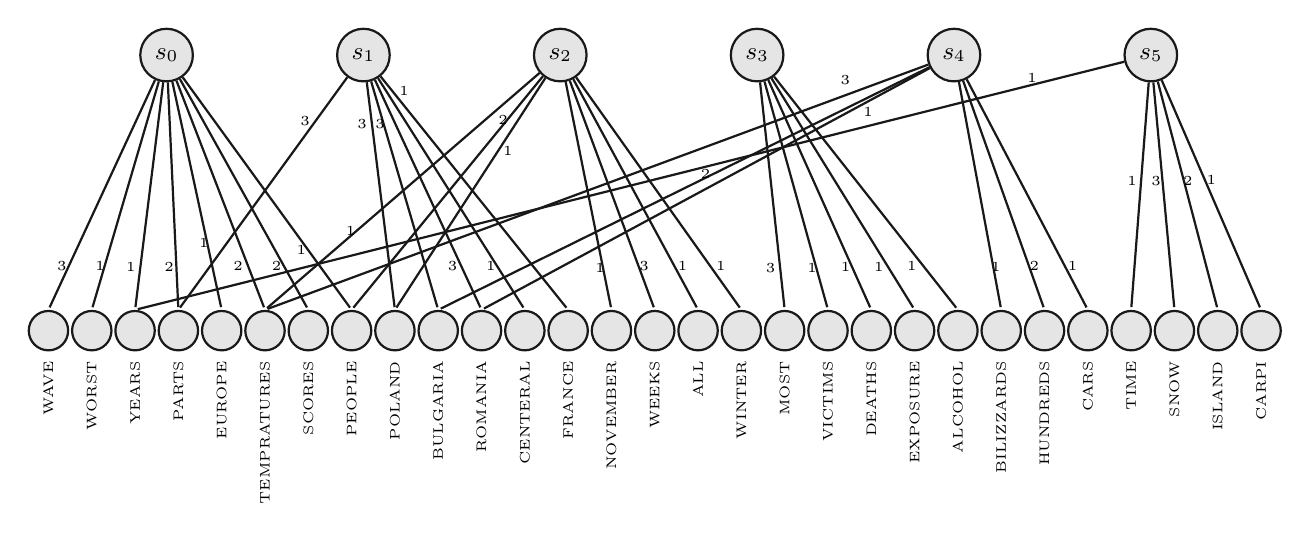
\begin{tikzpicture}[shorten >=1pt,-,scale=0.5]  
				
				\tikzstyle{sentence}=[circle,thick,draw=black!90,fill=black!10,minimum size=2mm]
				\tikzstyle{entity}=[circle,thick,draw=black!90,fill=black!10,minimum size=5mm]
				\tikzstyle{edge}=[draw=black!90, thick]
			   
			   \begin{scope}
			   
				 \node [sentence] (s0) at (-3,0) {\small{$s_0$}};
				 \node [sentence] (s1) at (2,0) {\small{$s_1$}};
				 \node [sentence] (s2) at (7,0) {\small{$s_2$}}; 
				 \node [sentence] (s3) at (12,0) {\small{$s_3$}}; 
				 \node [sentence] (s4) at (17,0) {\small{$s_4$}};
				 \node [sentence] (s5) at (22,0) {\small{$s_5$}}; 

				 \node [entity, label=below:\rotatebox{+90}{\tiny{WAVE}}] (e0)  at (-6.0,-7) {}; 
				 \node [entity, label=below:\rotatebox{+90}{\tiny{WORST}}] (e1)  at (-4.9,-7) {};
				 \node [entity, label=below:\rotatebox{+90}{\tiny{YEARS}}] (e2)  at (-3.8,-7) {}; 
				 \node [entity, label=below:\rotatebox{+90}{\tiny{PARTS}}] (e3)  at (-2.7,-7) {}; 
				 \node [entity, label=below:\rotatebox{+90}{\tiny{EUROPE}}] (e4)  at (-1.6,-7) {}; 
				 \node [entity, label=below:\rotatebox{+90}{\tiny{TEMPRATURES}}] (e5)  at (-0.5,-7) {}; 
				 \node [entity, label=below:\rotatebox{+90}{\tiny{SCORES}}] (e6)  at (0.6,-7) {}; 
				 \node [entity, label=below:\rotatebox{+90}{\tiny{PEOPLE}}] (e7)  at (1.7,-7) {}; 
				 \node [entity, label=below:\rotatebox{+90}{\tiny{POLAND}}] (e8)  at (2.8,-7) {}; 
				 \node [entity, label=below:\rotatebox{+90}{\tiny{BULGARIA}}] (e9)  at (3.9,-7) {}; 
				 \node [entity, label=below:\rotatebox{+90}{\tiny{ROMANIA}}] (e10)  at (5.0,-7) {}; 
				 \node [entity, label=below:\rotatebox{+90}{\tiny{CENTERAL}}] (e11)  at (6.1,-7) {}; 
				 \node [entity, label=below:\rotatebox{+90}{\tiny{FRANCE}}] (e12)  at (7.2,-7) {}; 
				 \node [entity, label=below:\rotatebox{+90}{\tiny{NOVEMBER}}] (e13)  at (8.3,-7) {}; 
				 \node [entity, label=below:\rotatebox{+90}{\tiny{WEEKS}}] (e14)  at (9.4,-7) {}; 
				 \node [entity, label=below:\rotatebox{+90}{\tiny{ALL}}] (e15)  at (10.5,-7) {}; 
				 \node [entity, label=below:\rotatebox{+90}{\tiny{WINTER}}] (e16)  at (11.6,-7) {}; 
				 \node [entity, label=below:\rotatebox{+90}{\tiny{MOST}}] (e17)  at (12.7,-7) {}; 
				 \node [entity, label=below:\rotatebox{+90}{\tiny{VICTIMS}}] (e18)  at (13.8,-7) {}; 
				 \node [entity, label=below:\rotatebox{+90}{\tiny{DEATHS}}] (e19)  at (14.9,-7) {}; 
				 \node [entity, label=below:\rotatebox{+90}{\tiny{EXPOSURE}}] (e20)  at (16.0,-7) {}; 
				 \node [entity, label=below:\rotatebox{+90}{\tiny{ALCOHOL}}] (e21)  at (17.1,-7) {}; 
				 \node [entity, label=below:\rotatebox{+90}{\tiny{BILIZZARDS}}] (e22)  at (18.2,-7) {}; 
				 \node [entity, label=below:\rotatebox{+90}{\tiny{HUNDREDS}}] (e23)  at (19.3,-7) {}; 
				 \node [entity, label=below:\rotatebox{+90}{\tiny{CARS}}] (e24)  at (20.4,-7) {}; 
				 \node [entity, label=below:\rotatebox{+90}{\tiny{TIME}}] (e25)  at (21.5,-7) {}; 
				 \node [entity, label=below:\rotatebox{+90}{\tiny{SNOW}}] (e26)  at (22.6,-7) {}; 
				 \node [entity, label=below:\rotatebox{+90}{\tiny{ISLAND}}] (e27)  at (23.7,-7) {}; 
				 \node [entity, label=below:\rotatebox{+90}{\tiny{CARPI}}] (e28)  at (24.8,-7) {}; 

				 
				 \path[edge] (s0) edge [above, very near end] node[font=\tiny] {$3$} (e0.north); %, line width=0.3ex
				 \path[edge] (s0) edge [above, very near end] node[font=\tiny] {$1$} (e1.north);
				 \path[edge] (s0) edge [above, very near end] node[font=\tiny, xshift=-1mm] {$1$} (e2.north);
				 \path[edge] (s0) edge [above, very near end] node[font=\tiny, xshift=-1mm] {$2$} (e3.north);
				 \path[edge] (s0) edge [above, very near end] node[font=\tiny, yshift=3mm, xshift=-1.5mm] {$1$} (e4.north);
				 \path[edge] (s0) edge [above, very near end] node[font=\tiny, xshift=-2mm] {$2$} (e5.north);
				 \path[edge] (s0) edge [above, very near end] node[font=\tiny, xshift=-2mm] {$2$} (e6.north);
				 \path[edge] (s0) edge [above, very near end] node[font=\tiny, yshift=2mm, xshift=-3.7mm] {$1$} (e7.north);

				 \path[edge] (s1) edge [above, near start] node[font=\tiny, near start] {$3$} (e3.north);
				 \path[edge] (s1) edge [above, near start] node[font=\tiny, xshift=-1.5mm] {$3$} (e8.north);
				 \path[edge] (s1) edge [above, near start] node[font=\tiny, xshift=-1mm] {$3$} (e9.north);
				 \path[edge] (s1) edge [above, very near end] node[font=\tiny, xshift=-2mm] {$3$} (e10.north);
				 \path[edge] (s1) edge [above, very near end] node[font=\tiny, xshift=-2mm] {$1$} (e11.north);
				 \path[edge] (s1) edge [above, very near start] node[font=\tiny] {$1$} (e12.north);

				 \path[edge] (s2) edge [above, very near end] node[font=\tiny, yshift=4.4mm, xshift=6.5mm] {$1$} (e5.north);
				 \path[edge] (s2) edge [above, near start] node[font=\tiny, xshift=1mm] {$2$} (e7.north);
				 \path[edge] (s2) edge [below, near start] node[font=\tiny] {$1$} (e8.north);
				 \path[edge] (s2) edge [below,  near end] node[font=\tiny] {$1$} (e13.north);
				 \path[edge] (s2) edge [above, very near end] node[font=\tiny] {$3$} (e14.north);
				 \path[edge] (s2) edge [above, very near end] node[font=\tiny] {$1$} (e15.north);
				 \path[edge] (s2) edge [above, very near end] node[font=\tiny] {$1$} (e16.north);

				 \path[edge] (s3) edge [below,  near end] node[font=\tiny,xshift=-1mm] {$3$} (e17.north);
				 \path[edge] (s3) edge [below,  near end] node[font=\tiny] {$1$} (e18.north);
				 \path[edge] (s3) edge [below,  near end] node[font=\tiny] {$1$} (e19.north);
				 \path[edge] (s3) edge [below,  near end] node[font=\tiny] {$1$} (e20.north);
				 \path[edge] (s3) edge [below,  near end] node[font=\tiny] {$1$} (e21.north);

				 \path[edge] (s4) edge [above, very near start] node[font=\tiny] {$3$} (e5.north);
				 \path[edge] (s4) edge [below, very near start] node[font=\tiny] {$1$} (e9.north);
				 \path[edge] (s4) edge [above, midway] node[font=\tiny] {$2$} (e10.north);
				 \path[edge] (s4) edge [above, very near end] node[font=\tiny] {$1$} (e22.north); 
				 \path[edge] (s4) edge [above, very near end] node[font=\tiny] {$2$} (e23.north); 
				 \path[edge] (s4) edge [above, very near end] node[font=\tiny] {$1$} (e24.north);     

				 \path[edge] (s5) edge [above, very near start] node[font=\tiny, xshift=4mm] {$1$} (e2.north);
				 \path[edge] (s5) edge [above, midway] node[font=\tiny,xshift=-1mm] {$1$} (e25.north);
				 \path[edge] (s5) edge [above, midway] node[font=\tiny,xshift=-1mm] {$3$} (e26.north);
				 \path[edge] (s5) edge [above, midway] node[font=\tiny] {$2$} (e27.north); 
				 \path[edge] (s5) edge [above, midway] node[font=\tiny] {$1$} (e28.north);   

				\end{scope}        
			  \end{tikzpicture}
		\end{tabular}
		}%
	\end{center}
	\caption{The entity graph representation of the text presented in Example \ref{ex:rel-text}. 
	The graph is obtained from the entity grid representation shown in Table \ref{tab:rel-egrid}. 
	The top nodes represent columns in the gird or sentences in the text. 
	The bottom nodes capture rows in the grid or entities in the text. 
	Edges encode the entries in the grid. 
	Weights of edges represent the value of each entry in the gird: 3:S, 2:O, 1:X, and 0:--. 
	The weight of 0 is equivalent with no edge in a graph, so they are not drawn in the graph.  
	}
	\label{fig:rel-egraph}
\end{figure}

\subsubsection{Coherence Measurement: The Average Outdegree of Projection Graphs}

\paragraph{Projection graphs.}
Local coherence is about the connectivity among sentences in a text. 
Sentences are modeled by one set of nodes in the entity graph representation, and the other set of nodes captures entities. 
\newcite{guinaudeau13} propose to transfer entity graphs to a graph whose nodes capture only sentences, and relations encode entity-based connections between sentences. 
Such a graph, which is obtained from a bipartite graph, is called a one-mode projection graph (or a projection graph for the sake of brevity) in the graph theory \cite{newmanmark10}. 
Edges in projection graphs can be weighted in different ways in order to retain specific information about  relations between sentence nodes and entity nodes in the entity graph. 
Moreover, edges in projection graphs are directed to encode the order of sentences in a text. 

\newcite{guinaudeau13} apply three kinds of projections, namely $P_U$, $P_W$ and $P_{Acc}$. 
Figure \ref{fig:rel-proj} shows these graphs obtained from the entity graph presented in Figure \ref{fig:rel-egraph}. 
These projection graphs differ in the weighting scheme that is associated with their edges: 

\begin{itemize}

	\item In $P_U$, weights are binary, i.e.\ 0 or 1. 
	The weight of an edge between two nodes in this type of the projection graph is equal to $1$ if the sentence nodes are connected to at least one entity node in the entity graph.  
	This projection graph merely captures which sentences are linked to each other in a text. 

	\item In $P_W$, an edge is weighted according to the number of the entity nodes that are connected with both sentence nodes in the entity graph. 
	In other words, the weight of an edge between two nodes in this type of the projection graph represents the number of shared entities by the corresponding sentences. 
	This projection graph not only models which sentences are connected to each other but how strongly  sentences are related. 
	It takes the number of common entities between a pair of sentences as the strength of the relation between sentences. 

	\item In $P_{Acc}$ syntactic information is accounted for by integrating the edge weights in the entity graph. 
	In this case, the weight of the edge between nodes $s_i$ and $s_k$ is equal to

	\begin{equation}
		W_{ik} = \sum_{e \in E_{ik}}{w(e,s_i) \cdot w(e,s_k)},
	\end{equation}
	%
	where $E_{ik}$ is the set of the entity nodes that are connected to both $s_i$ and $s_k$. 
	This type of the projection graph incorporates grammatical information about shared entities by sentences in order to measure the strength of the relation between sentences. 

\end{itemize}


\begin{figure}[!ht]
	\begin{center}
		\begin{tabular}{@{}lc@{}}
			\begin{tikzpicture}        
					 \node [] (n0) at (0,0) {};
			         \node [] (label) at (0,0.8) {$P_U:$};
			\end{tikzpicture}
			&
			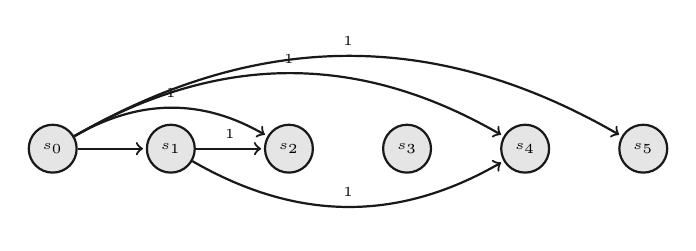
\begin{tikzpicture}[shorten >=1pt,->,scale=0.5]  
        		\tikzstyle{sentence}=[circle,thick,draw=black!90,fill=black!10,minimum size=2mm]
				\tikzstyle{entity}=[circle,thick,draw=black!90,fill=black!10,minimum size=2mm]
        		\tikzstyle{edge}=[draw=black!90, thick]

       			\begin{scope}

			         \node [sentence] (s0) at (0,0) {\tiny{$s_0$}};
			         \node [sentence] (s1) at (3,0) {\tiny{$s_1$}};
			         \node [sentence] (s2) at (6,0) {\tiny{$s_2$}}; 
			         \node [sentence] (s3) at (9,0) {\tiny{$s_3$}}; 
			         \node [sentence] (s4) at (12,0) {\tiny{$s_4$}};
			         \node [sentence] (s5) at (15,0) {\tiny{$s_5$}}; 
 
			 		\path[edge] (s0) edge [above] node[font=\tiny]{} (s1);
			 		\path[edge, bend left = 30] (s0) edge [above] node[font=\tiny]{$1$} (s2);
					\path[edge, bend left = 30] (s0) edge [above] node[font=\tiny]{$1$} (s4);
			 		\path[edge, bend left = 30] (s0) edge [above] node[font=\tiny]{$1$} (s5);

			 		\path[edge] (s1) edge [above] node[font=\tiny]{$1$} (s2);
					\path[edge, bend right = 30] (s1) edge [above] node[font=\tiny]{$1$} (s4);
           
		        \end{scope}        
     		 \end{tikzpicture}

			 \\

			\begin{tikzpicture}        
				 \node [] (n0) at (0,0) {};
        		 \node [] (label) at (0,0.8) {$P_W:$};
			\end{tikzpicture}
 			&
			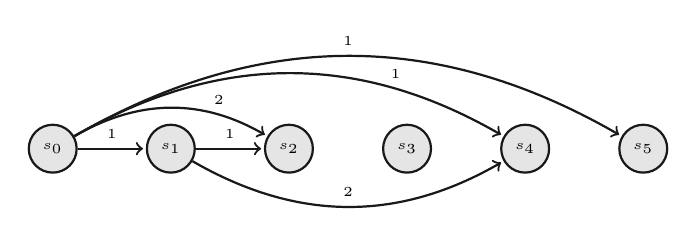
\begin{tikzpicture}[shorten >=1pt,->,scale=0.5]  
        			\tikzstyle{sentence}=[circle,thick,draw=black!90,fill=black!10,minimum size=2mm]
					\tikzstyle{entity}=[circle,thick,draw=black!90,fill=black!10,minimum size=2mm]
			        \tikzstyle{edge}=[draw=black!90, thick]
 			 
 			       \begin{scope}
       
     				    \node [sentence] (s0) at (0,0) {\tiny{$s_0$}};
				         \node [sentence] (s1) at (3,0) {\tiny{$s_1$}};
				         \node [sentence] (s2) at (6,0) {\tiny{$s_2$}}; 
				         \node [sentence] (s3) at (9,0) {\tiny{$s_3$}}; 
				         \node [sentence] (s4) at (12,0) {\tiny{$s_4$}};
				         \node [sentence] (s5) at (15,0) {\tiny{$s_5$}}; 
				 
				 		\path[edge                ] (s0) edge [above, midway] node[font=\tiny]{$1$} (s1);
				 		\path[edge, bend left = 30] (s0) edge [above, near end] node[font=\tiny]{$2$} (s2);
						\path[edge, bend left = 30] (s0) edge [above, near end] node[font=\tiny]{$1$} (s4);
				 		\path[edge, bend left = 30] (s0) edge [above, midway] node[font=\tiny]{$1$} (s5);

				 		\path[edge                 ] (s1) edge [above, midway] node[font=\tiny]{$1$} (s2);
						\path[edge, bend right = 30] (s1) edge [above, midway] node[font=\tiny]{$2$} (s4);
           
    			    \end{scope}        
   		   \end{tikzpicture}

			\\

			\begin{tikzpicture}        
				 \node [] (n0) at (0,0) {};
		         \node [] (label) at (0,0.8) {$P_{Acc}:$};
			\end{tikzpicture}
 			&

		   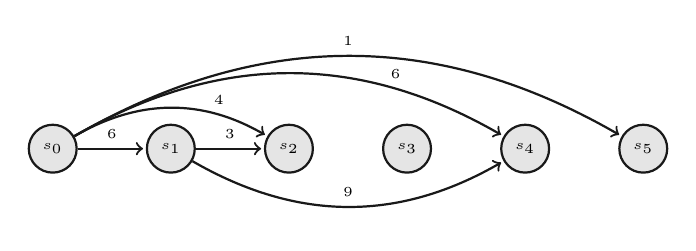
\begin{tikzpicture}[shorten >=1pt,->,scale=0.5]  
		        \tikzstyle{sentence}=[circle,thick,draw=black!90,fill=black!10,minimum size=2mm]
				\tikzstyle{entity}=[circle,thick,draw=black!90,fill=black!10,minimum size=2mm]
		        \tikzstyle{edge}=[draw=black!90, thick]

		        \begin{scope}

			         \node [sentence] (s0) at (0,0) {\tiny{$s_0$}};
			         \node [sentence] (s1) at (3,0) {\tiny{$s_1$}};
			         \node [sentence] (s2) at (6,0) {\tiny{$s_2$}}; 
			         \node [sentence] (s3) at (9,0) {\tiny{$s_3$}}; 
			         \node [sentence] (s4) at (12,0) {\tiny{$s_4$}};
			         \node [sentence] (s5) at (15,0) {\tiny{$s_5$}}; 
 
			 		\path[edge                ] (s0) edge [above, midway] node[font=\tiny]{$6$} (s1);
			 		\path[edge, bend left = 30] (s0) edge [above, near end] node[font=\tiny]{$4$} (s2);
					\path[edge, bend left = 30] (s0) edge [above, near end] node[font=\tiny]{$6$} (s4);
			 		\path[edge, bend left = 30] (s0) edge [above, midway] node[font=\tiny]{$1$} (s5);

			 		\path[edge                 ] (s1) edge [above, midway] node[font=\tiny]{$3$} (s2);
					\path[edge, bend right = 30] (s1) edge [above, midway] node[font=\tiny]{$9$} (s4);
           
		        \end{scope}        
      
      		\end{tikzpicture}

		\end{tabular}
	\end{center}
	\caption{
	Three types of projection graphs that are employed by the entity graph model. 
	$P_U$ shows only which sentence nodes are connected. 
	$P_W$ takes the number of shared entities as the weight of edges. 
	$P_{Acc}$ involves grammatical roles of common entities between sentences. 
	}
	\label{fig:rel-proj}
\end{figure}

Distances between sentences can be integrated in the weighting scheme of edges in the projection graphs to decrease the importance of links between non-adjacent sentences \cite{guinaudeau13}.   
In this case, edge weights in projection graphs are divided by the number of sentences in between of two sentences. 

\paragraph{The average outdegree as a coherence metric.}
Given a projection graph representation of a text, the coherence of the text can be measured based on the connectivity of nodes in the projection graph. 
\newcite{guinaudeau13} assume that projection graphs of coherent texts contain more edges than the projection graph of incoherent ones.  
They propose to use a centrality metric \cite{newmanmark10} in the graph theory for measuring to what extend nodes in a projection graph are connected with each other. 
Let $outdegree(s)$ be the sum of the weights associated to edges that leave node $s$ in projection graph $P$, then the centrality metric of the projection graph is computed by the average outdegree of all nodes ($N$) in the graph: 

\begin{equation}
	 AvgOutDeg(P) = \frac{1}{N} \sum_{i=1}^{N} outDegree(s_i).
\end{equation}

Table \ref{tab:rel-od} shows the AvgOutDeg for different projection graphs presented in Figure \ref{fig:rel-proj}. 

\begin{table}[!ht]
	\begin{center}
		\begin{tabular}{ll}
			\hline
			 $P$ & $ AvgOutDeg(P)$ \\\hline
			 $P_U$ & $\frac{1}{6} \left((1+1+1+1)+(1+1)+(0)+(0)+(0)+(0)) \right) = 1.00$ \\
			 $P_W$ & $\frac{1}{6} \left((1+2+1+1)+(1+2)+(0)+(0)+(0)+(0)) \right) = 1.33$\\
			 $P_{Acc}$ &$\frac{1}{6} \left((6+4+6+1)+(3+9)+(0)+(0)+(0)+(0)) \right) = 4.83$ \\
			 $P_U\textit{, }Dist$ & $\frac{1}{6} \left((1+0.50+0.25+0.20)+(1+0.33)+(0)+(0)+(0)+(0)) \right) = 0.55$ \\
			 $P_W\textit{, }Dist$ & $\frac{1}{6} \left((1+1+0.25+0.20)+(1+0.66)+(0)+(0)+(0)+(0)) \right)= 0.69$ \\
			 $P_{Acc}\textit{, }Dist$ & $\frac{1}{6} \left((6+2+1.5+0.2)+(3+3)+(0)+(0)+(0)+(0)) \right)= 2.61$ \\
			 \hline
		\end{tabular}
	\end{center}
	\caption{The average outdegree of nodes in projection graphs presented in Figure \ref{fig:rel-proj}.}
	\label{tab:rel-od}
\end{table}

In order to rank a pair of texts with respect to their coherence, \newcite{guinaudeau13} represent both texts with the same type of projection graphs, and then use the average outdegree of their projection graphs to compare texts. 
It is worth to mention that the proposed entity graph model by \newcite{guinaudeau13} is an unsupervised model because the final average outdegree is directly employed for comparing two texts with respect to their coherence. 
However, average outdegree captures no information about the connectivity style of nodes in a projection graph. 
For example consider two projection graphs that are shown in Figure \ref{fig:rel-avgod-weakness}. 
These two graphs have the same average outdegree, i.e.\ five, but graph (b) is disconnected because node $s_2$ is not connected to its preceding nodes. The outdegree does not capture such information about the connectivity of nodes. 

\begin{figure}[!ht]
	\begin{center}
		\begin{tabular}{@{}c@{}}
			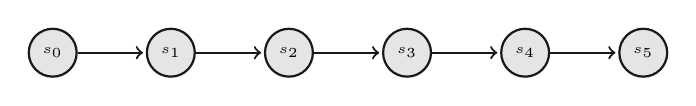
\begin{tikzpicture}[shorten >=1pt,->,scale=0.5]  
        		\tikzstyle{sentence}=[circle,thick,draw=black!90,fill=black!10,minimum size=2mm]
				\tikzstyle{entity}=[circle,thick,draw=black!90,fill=black!10,minimum size=2mm]
        		\tikzstyle{edge}=[draw=black!90, thick]

       			\begin{scope}

			         \node [sentence] (s0) at (0,0) {\tiny{$s_0$}};
			         \node [sentence] (s1) at (3,0) {\tiny{$s_1$}};
			         \node [sentence] (s2) at (6,0) {\tiny{$s_2$}}; 
			         \node [sentence] (s3) at (9,0) {\tiny{$s_3$}}; 
			         \node [sentence] (s4) at (12,0) {\tiny{$s_4$}};
			         \node [sentence] (s5) at (15,0) {\tiny{$s_5$}}; 
 
			 		\path[edge] (s0) edge (s1);
			 		\path[edge] (s1) edge (s2);
			 		\path[edge] (s2) edge (s3);
			 		\path[edge] (s3) edge (s4);
			 		\path[edge] (s4) edge (s5);
			 		
		        \end{scope}        
     		 \end{tikzpicture}
     		\\
     			(a) A projection graph with the outdegree of five, and all nodes are in one component. 
			\\
			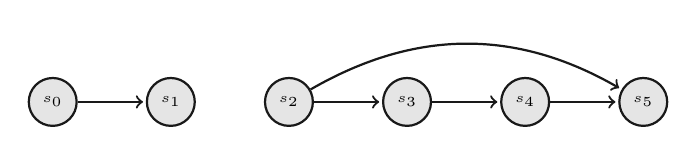
\begin{tikzpicture}[shorten >=1pt,->,scale=0.5]  
        			\tikzstyle{sentence}=[circle,thick,draw=black!90,fill=black!10,minimum size=2mm]
					\tikzstyle{entity}=[circle,thick,draw=black!90,fill=black!10,minimum size=2mm]
			        \tikzstyle{edge}=[draw=black!90, thick]
                  \begin{scope}

			         \node [sentence] (s0) at (0,0) {\tiny{$s_0$}};
			         \node [sentence] (s1) at (3,0) {\tiny{$s_1$}};
			         \node [sentence] (s2) at (6,0) {\tiny{$s_2$}}; 
			         \node [sentence] (s3) at (9,0) {\tiny{$s_3$}}; 
			         \node [sentence] (s4) at (12,0) {\tiny{$s_4$}};
			         \node [sentence] (s5) at (15,0) {\tiny{$s_5$}}; 
 
			 		\path[edge] (s0) edge (s1);
			 		
			 		\path[edge] (s2) edge (s3);
			 		\path[edge] (s3) edge (s4);
			 		\path[edge] (s4) edge (s5);
			 		\path[edge, bend left = 30] (s2) edge (s5);
                  \end{scope}
   		   \end{tikzpicture}
   		   \\ 
   		   (b) A projection graph with the outdegree of five with two components. 
		\end{tabular}
	\end{center}
	\caption{}
	\label{fig:rel-avgod-weakness}
\end{figure}

Moreover, there are three types of projection graphs that behave differently in different tasks. 
So it is not clear finally which type of projection graphs should be employed to be used in a downstream task. 

\subsubsection{Extensions of the Entity Graph Model}

The entity graph model is extended from different perspectives: text representation, and the graph metric that is employed for coherence measurement. 

\newcite{petersen15} use several graph metrics, rather than the average outdegree, to approximate different aspects of the text flow that can indicate coherence.  
These metrics are designed to capture more information about the connectivity style of nodes in projection graphs. 
For example, they use the mean of the PageRank scores \cite{newmanmark10}  of nodes in a projection graph to distinguish between a star-graph, in which all nodes are connected to one node and no other edges occur; and a path graph, in which all nodes occur in a chain. 
Other assessed metrics include a clustering coefficient, which measures to which extent neighbors of a node are connected among themselves; betweenness, which is the fraction of shortest paths that contain a node, and etc. 
Although their results are better than the original entity graph but the difference is not considerable to use these metrics, especially when the average outdegree is easy and efficient to compute. 
% \newcite{dias15} propose to fill the grid in the entity grid based on the RST relations between sentences in a text. 
% An entry in the entity grid is one if an entity is part of a sentence that participate in a RST relation.
% Similarly they define a bipartite graph as its original version and use outdegree to measure coherence of texts. 
% Their model outperforms the entity graph model. 
% However, similar to RST-based extensions of the entity grid model, they argue that obtaining RST relations is subjective, and human annotation or a discourse parser is not available for many languages. 

\newcite{zhangmuyu15} use the semantic relations between named entities to not only cover 
the mentions that refer to the same entity but also the mentions that refer to entities which are semantically related (e.g.\ Gates and Microsoft). 
They capture such semantic relations by leveraging WordNet \cite{baccianella10} as a knowledge base. 
They limit the semantic relation between entities to argument$_1$-predicate-argument$_2$, such as Gates-create-Microsoft. 
The performance of both the entity graph model is improved by incorporating these relations. 
They also challenge the average outdegree metric that is used to measure the coherence of a text. 
They propose to combine average outdegree with another score named reachability. 
The reachability score is the sum of the weights from the first sentence node to the current sentence node. 
The intuition behind the reachability score of nodes is that this score reflects the tightness between this sentence and the preceding part of the text. 


We propose\footnote{We just briefly explain this model here because it does not focus on coherence patterns which are the core of the research presented in this thesis.} \cite{mesgar14} an extension of the entity graph model by taking the entity and sentence importance into account. 
We try to reflect the structure of connections in an entity graph into the weights of edges in the graph by applying a normalization method to edge weights.  
The normalization method reduces the difference in performance of three types of projection graphs by combining the information in these graphs. 

% \newcite{lioma16} eliminate the need for the projection graph with this intuition that projection incur significant loss of information present in an entity graph.  
% They present three new graph metrics that measure text coherence directly based on entity graphs. 
% These metrics are obtained by different ways of normalizing the weights of the entity graph representation. 
%As a result methods that rely on strict entity matching would fail on these cases. 

\section{Lexical Approaches to Local Coherence}

An important factor in text comprehension is the degree to which sentences are linked together. 
\newcite{halliday76} stressed the role of lexical cohesion in text coherence. 
A number of linguistic devices —- repetition, synonymy, hyponymy, meronymy, and etc —- are considered to contribute to the ``continuity of lexical meaning'' observed in coherent text. 
In this section, we mainly survey the computational models that use lexical relations for modeling local coherence. 
However, since these models are based on the lexico-semantic relations between words in a text, we first discuss different resources that are used in literature to recognize these relations. 

\subsection{Lexical Resources} 

Most lexical models in natural language processing crucially rely on the existence of resources that encode information about semantic relations between words in a language. 
Such resources are typically acquired via two main approaches: the knowledge-based approach, or top–down, where information is manually curated by humans, and the corpus-based approach, or bottom–up, where information is automatically learned from corpora. 
Although the latter has gained ground during the last decade — benefiting from the availability of large amounts of text and from increased computing capacities, the former remains fundamental for it allows us to collect reliable, fine-grained, and explicit information. 

\paragraph{Knowledge-based resources.}
One of the fundamental lexical knowledge resources for English is the Princeton WordNet \cite{fellbaum98}.  
This WordNet aims to represent real-world concepts and relations between them as they are commonly perceived by humans. 
It covers about 20 million instances extracted from row texts. 
Nouns, verbs, adjectives, and adverbs are each organized into networks of synonym sets (synsets) that each represent one underlying lexical concept and are interlinked with a variety of relations. 
WordNet-based similarity measures have been shown to correlate reliably with human similarity judgments and have been used in a variety of applications ranging from the detection of malapropisms to word sense disambiguation \cite{budanitsky06}.  
The Princeton WordNet for English inspired the creation of a lexical knowledge base in some other languages such as German, which is called GermanNet \cite{hamp97}. 
However, it is not still available for many languages because it needs human experts for annotations.  
YAGO \cite{hoffart13} is another instance of knowledge resources.  
It consists of four million instances that are automatically extracted from online encyclopedias such as WikiPedia \cite{denoyer06} and FreeBase \cite{bollacker08}. 
Relations then are edited by humans. 
Generally speaking, manually edited knowledge bases have better accuracy but lower coverage, while automatically extracted knowledge bases are the opposite. 

These knowledge bases are employed by different coherence models \cite{lapata05a,zhangmuyu15}. 
\newcite{zhangmuyu15} explain two major issues for retrieving world knowledge related to words in a text: 
\begin{itemize}
\item knowledge source: which resource is the best for obtaining this knowledge? 
\item knowledge selection: how do we pinpoint the most relevant entry in a knowledge base?
\end{itemize}
Knowledge resources cover semantic relations between certain sets of word categories.  
For example, WordNet is designed to provide complete coverage of common, open-class English words. 
Therefore, it has little or no coverage of vocabularies from specialized domains, and very limited coverage of proper nouns. 
This may hinder its application to domain-specific contexts and tasks required to deal with proper nouns. 
The issue related to knowledge selection is that if to retrieve knowledge instances using exact or partial matching. 
The chance of exact matching of words (especially entities) in a text with instances in knowledge base is low \cite{zhangmuyu15}. 
In contrast, partial matching between arguments and entities usually increases coverage but at the risk of introducing some noise. 

In this type of knowledge resources, a simple way to compute the semantic relations between words is to view it as a graph. 
The semantic relatedness can be measured based on graph properties such as the path length between the words \cite{budanitsky06}. 
The shorter the path between two word nodes, the more similar the words are. 

\paragraph{Corpus-based resources.} 
The bottom-up knowledge resources are obtained based on the co-occurance of words in texts in corpora. 
In these resources, words are considered similar if they occur within similar contexts. 
The semantic properties of words are captured in a multi-dimensional space by vectors that are constructed from large bodies of texts by observing the distributional patterns of co-occurrence with their neighboring words. 
The semantic relatedness between words is then measured by the similarity between their corresponding vectors. 
These type of knowledge sources are different in terms of the method that is employed to obtain vector representations for words. 
One of the early techniques is Latent Semantic Analysis (LSA) proposed by \newcite{landauer97}. 
This method construct a matrix, namely occurrence matrix, containing word counts per text from a large number of texts in a corpora.  
It then uses a mathematical technique called singular value decomposition (SVD) \cite{} to reduce the text dimensionality in the matrix while preserving the similarity structure among words. 
% LSA involves the application of Singular Value Decomposition to the document-by-term matrix in order to reduce its rank. 
% Because information is lost in this compassion process, some similar vectors will be conflated, or moved closer whiting the space. 
% LSA has proved to be a great improvement over the simple vector-space IR model for some domains. 
% The term-term similarity scores it produces are more robust (Landauer et al., 1998, Haggins and Burstein (2007)).
% LSA has been shown to be applicable to the task of establishing text coherence (Foltz et al. (1998)) although their application of LSA in this domain is very different from ours. 
% There were some drawbacks with LSA models that do not exist in these days. 
% For one thing, Singular Value Decomposition requires a numerical computation which is demanding both good possessing units and memory units. 
% LSA is also very dependent on the corpus used to train it. 
% Since term-occurrence within. documents is the basis for the generalizations it derives, it performs best when trained on corpora which are very topically coherent and which cover a diverse set of topics. 
% An encyclopedia is a good text to use for LSA, but it is hard to obtain high quality encyclopedic texts as low cost, especially in large quantity. 
% Random Indexing is more efficient method than LSA for term similarity. 
% %% TO DO: what are some draw backs of LSA? why should we use word embeddings?


The other method is Latent Dirichlet allocation (LDA) proposed by \newcite{blei03}. 
It is a generative statistical model that allows sets of words to be explained by latent topic groups that explain why some parts of a text are similar. 
This method is identical to probabilistic latent semantic analysis (pLSA), except that in LDA the topic distribution is assumed to have a sparse Dirichlet prior.
The sparse Dirichlet priors encode the intuition that documents cover only a small set of topics and that topics use only a small set of words frequently. 
In practice, this results in a better disambiguation of words and a more precise assignment of documents to topics.
A topic is neither semantically nor epistemologically strongly defined. 
It is identified on the basis of automatic detection of the likelihood of term co-occurrence. 
A lexical word may occur in several topics with a different probability, however, with a different typical set of neighboring words in each topic.

Finally, recent methods for representing words in a distributional space use deep neural networks, rather than co-occurrence matrix. 
In contrast to the primary methods that are unsupervised, the neural network models applied for obtaining word vectors are supervised.  
This property is an advantage for these methods because as the vocabulary in a language grows new vectors for new vocabulary can be trained and added to the knowledge base. 
The word vectors that are generated by these models are named word embeddings. 
Well-know approaches for obtaining word embedding are \emph{word2vec}  \cite{mikolov13} and \emph{GloVe} \cite{pennington14}. 
The word2vec approach focuses on learning the embeddings of a word given its local usage context, where the context is defined by a window of surrounding words. 
This window is a configurable parameter of the model. 
Large windows tend to produce more topical similarities and smaller windows tend to produce more functional and syntactic similarities \cite{goldberg17}. 
The GloVe approach constructs an explicit word-context or word co-occurrence matrix using statistics across the whole text corpus, rather than using a window to define local context. 
Indeed, word embeddings are useful if they are trained on sufficiently large and balance corpora.; otherwise there is a risk \cite{lindekang98b} of finding words which their similarity only makes sense in the corpus that is used. 
\newcite{budanitsky06} highlight other problems that arise from the imbalance and sparseness of corpora.

In bottom-up recourses such as pre-trained word embeddings, words are compared by taking the cosine of the angle between the two vectors (or the dot product between the normalizations of the two vectors). Values close to 1 represent very semantically close words while values close to 0 represent very distant words. 

\subsection{Lexical Cohesion Models}

Lexical chain has a long history in local coherence modeling for different applications \cite{benguosheng13,wongbillytm12,fenglijun09,flor13}. 
Pioneering work \cite{morris91,hirst95} in coherence modeling based on lexical relations between words, or lexical cohesion, focus on lexical chaining. 
A lexical chain is a sequence of semantically related words spanning a topical text unit. 
Semantic relations are induced from Roget's Thesaurus. 
The thesaurus offers a structural account of the vocabulary of English, grouping into a hierarchical  categories. 
The main intuition behind this work is that coherent texts have a high concentration of dense chains. 
Therefore, the distribution of lexical chains is a surface indicator of the structure of coherent discourse. 
\newcite{galley03} also use lexical chains, but those are built simply based on word repetition. 
Therefore this model does need any knowledge resources.  
They define different features of lexical chains such as length of chains. 
In contrast, \newcite{stokes04} employ WordNet to extract lexical chains from texts.  
Weak relations between words in lexical chains in a text is used as an indicator of topic shifts in the text. 
\newcite{barzilay97} propose a lexical chaining algorithm which uses WordNet, thesaurus, and pos tags to extract lexical relations. 
However, they do not use this model directly for coherence modeling but they utilize it for generating coherent summaries. 
\newcite{somasundaran14} use lexical chaining for measuring the quality of essays written by students. 
To do so, they employ Lin’s thesaurus \cite{lindekang98} to identify semantically similar words in essays.   
The main intuition is that the number of chains and their properties reveal coherence of texts in terms of focus in topic and elaboration. 
The attributes that they employ capture different aspect of lexical chains such the chain size, the number of chains that contain more than one word type, and so forth. 
% \newcite{benguosheng13} propose a bilingual lexical cohesion model for document-level machine translation.  
% The coherence of the translated document is achieved by considering lexical cohesion items in the source document. 
% The idea is that the strength of the semantic relation between two words should be retained in their counterparts in the translated document. 
% In this way the translated document is easier to read if the source document is readable. 
% \newcite{wongbillytm12} integrate lexical cohesion in assessment of translated documents. 
% Lexical cohesion items in a translated document should be ideally similar to those in its associated human translation. 
% In a closely related study, \newcite{fenglijun09} use lexical chains to measure readability. 
% Lexical chain features are employed to indicate the number of entities/concepts that a reader must keep in mind while reading a document.  
% \newcite{flor13} present a coherence model based on lexical tightness among content words in a text. 
% Lexical tightness represents the degree to which a text tends to use words that are highly inter-associated in a language. 
% They show that lexical tightness strongly correlates with readability level of expertly rated reading materials. 
% % Lexical chaining has been used in a number of applications such as news segmentation (Stokes, 2003), question-answering (Moldovan and Novischi, 2002), summarization (Barzilay and Elhadad, 1997), de- tection and correction of malapropisms (Hirst and St-Onge, 1995), topic detection (Hatch et al., 2000), topic tracking (Carthy and Sherwood-Smith, 2002), and keyword extraction (Ercan and Cicekli, 2007). 


Another trend in research regarding local coherence modeling considers lexical relations between words of sentences in order to compute the similarity between sentences.    
The main insight is that sentence in coherent texts are semantically similar. 
So these models represent each sentence by aggregating the vectors of its words, and the similarity between two sentences is determined by the similarity of their sentence vectors. 
Specifically, the coherence of a text is measured by taking the mean of all similarities between adjacent sentences in a text. 

\begin{equation}
coh(T) = \frac{\sum_{i=0}^{N-2}sim(s_i,s_{i+1})}{N-1},
\end{equation} 
%
where $sim(S_i, S_{i+1})$ is a measure of similarity between two adjacent sentences. 
This idea is operationalized in different ways.
For example, \newcite{foltz98} employ LSA to represent each word in a sentence by a vector and then use the weighted of word vectors to obtain sentence vectors. 
The weighting is inspired from information retrieval techniques, most notably TF-IDF, and performed by the log entropy transform of each word. 
The similarity between two adjacent sentences is computed by applying cosine function to sentence vectors. 
\newcite{barzilay0} compute the similarity between two adjacent sentences by counting the number of exact repetitions between nouns in sentences. 
\newcite{yannakoudakis12} measure local coherence based on different features including the lexical relations between sentences. 
They represent each sentence by vector of lemma/POS of words in sentences, and then the average of the cosine similarity between sentences encode how coherent the text is. 
\newcite{higgins07}  a similar strategy but sentences are represented by a Random Indexing model.
Other similar approaches are proposed by \cite{kazantseva14}. 
\newcite{hearst94, hearst97} compute the cosine similarity between adjacent window of words, rather than adjacent sentences. 

A recent trend of research uses the probabilistic models to assign a coherence sore to a text. 
\newcite{lapata03} proposes to compute the coherence probability between two adjacent sentence based on their lexical relations. 
This probability for a given pair of sentences is obtained by a conditional probability of words in a sentence given all words of its immediately preceding sentence. 
The coherence score of a text is the product of coherence probabilities between adjacent sentences. 
Although this model does not use any external knowledge resources but it computed its own co-occurrence matrix that captures words which occur in adjacent sentences. 
Moreover, this model is able to learn the order of word pairs, e.g. CAR precedes TIRE in coherent texts or vice versa. 
\newcite{lijiwei14} propose to represent words in sentences by pre-trained word embeddings, and then either recurrent or recursive neural networks are used to represent each sentence based on its word embeddings. 
A window with length three is sliding through a text and for each three adjacent sentences a coherence probability is computed. 
The final coherence sore of the text is obtained by multiplying these probabilities. 


\section{Coherence in Applications}
\label{sec:rel-coh-applications}

Coherence plays a crucial role in different natural language processing applications such as summarization \cite{}, information extraction \cite{}, essay analysis and scoring  \cite{burstein10}, sentiment analysis \cite{}, and assessing the readability of texts \cite{}. 
In this section, we review different tasks that have been employed for evaluating coherence models in the literature. 
We then explain why among these models, we choose readability assessment and text summarization for our evaluation purpose in this thesis. 
 
In order to evaluate a coherence model, a scoring function is required \cite{karamanis04}.   
A scoring function is a function that returns a score (or a set of scores) for the coherence of a text.  
This function is an increasing function; it returns higher scores for more coherent texts. 

Early work, which are inspired by Centering Theory, define different coherence functions based on the constraints introduced by Centering.    
For instance,  \newcite{poesio04, miltsakaku00}, as one of the informal Centering-based coherence scoring functions, propose a scoring function based on the number of each transition type in a text.  
The function returns higher scores for texts that have many number of CONTINUE transitions and less number of SHIFT transitions. 
\newcite{cheng02} present a genetic algorithm which handles the interaction between sentences.  
The scoring function uses the entity-based relations among sentences with features weighted according to preferences in Centering Theory.  
\newcite{kibble00} propose as scoring function based on the count the number of CT-based violations in texts. 
Texts with lower number of violations are more coherent. 

As it has been shown, CT is open-ended enough for one to propose new metrics which appear to be as plausible a some existing ones from a purely theoretical point of view. 
\newcite{karamanis04} explain that it is practically impossible to come up with an experimental design which accounts for the predictions of all aspects of coherence metrics at the same time. 

The entity grid coherence model \cite{barzilay05a} is evaluated on three tasks: sentence ordering, summary rating and readability assessment. 
In these tasks, coherence is taken as a relative property, rather than binary, of texts: Given a pairs of texts, which one is more coherent? 
They use a parametric scoring function based on the coherence features extracted from entity grid representations of texts.
Parameters of this function is trained by a machine learning approach so that the function best fits to the evaluation task and data. 
Therefore, the evaluation task should be designed in a way to model coherence difference between texts. 
Following \cite{barzilay05a}, other models \cite{} also use three tasks: sentence ordering, summary rating, and readability assessment. 

\subsubsection{Sentence Ordering}
It is known that the order of information in coherent texts is such that they are easy to follow \cite{lapata03,barzilay04,karamanis04b,barzilay05a,soricut06}. 
As it is explained in the definition of coherence, a text is more than a random concatenation of sentences; so the order of sentences affects how difficult the presented information in a text can be understood.  
Given the above fact, a document can be taken as an unordered bag of sentences and the task would be to find the ordering of the sentences that maximizes coherence according to a model. 
Unfortunately, finding the best ordering is NP-complete \cite{?} and non-approximable \cite{althaus04}.
Therefore, this task need to be simplified to be used for coherence evaluation. 
Two restricted versions of the sentence ordering tasks are the discrimination task, and the insertion task. 
In both subtasks the model is examined to see whether it is able to distinguish between the correct (original) order of sentences in a document and an incorrect (non-original) one. 

\paragraph{Discrimination.}
The discrimination task is based on this fact that the original order of sentences in a document is taken as the best order and any scrambling of sentences disturbs the perceived coherence of the document. 
By rearranging the order of sentences of a document, the document becomes more difficult to understand or less coherent, because the order of presented information is disturbed. 
More formally, let $COH_M(d)$ be the coherence estimation of document $d$ by the coherence model $M$ and $p$ be a version of $d$ that its sentences are randomly permuted, then the coherence model $M$ should ideally distinguish document $d$ a more coherent document than $p$:

\begin{equation}
COH_M(d) > COH_M(p). 
\end{equation}
where $COH_M$ is the scoring function defined by model $M$. 
\newcite{barzilay08} assume that the $COH_M(d)$ is a linear function of coherence features, which are defined as the entity transitions in the entity grid model, as follows:

\begin{equation}
COH_M(d) = \vec{w}^{T}.\vec{t}
\end{equation}

where $w$ is a vector of parameters, i.e.\ weights, and $t$ is the feature vector representing the coherence of $d$. 
The goal of the learning procedure is learn the best values for parameters $w$ in order to minimize the number of violations of pairwise rankings provided in the training set. 
The learning problem typically treated as a Support Vector Machine (SVM) constraint optimization problem, and can be solved using the search technique implemented in $SVM_{ligh}$\footnote{link to the package} \cite{joachims02} package. 
A model assigns local coherence values with the original document and its permutation, if the score for the original order of sentences of a document is higher than the score of the permutation version of sentence then the output of our system being considered correct. 
Because the relative quality of different permutations is unknown, the dataset includes only pairwise rankings that comprise the original document and one of its permutations.
Two evaluation metrics seem suitable for this task: accuracy and F-measure. 
Accuracy measures how correctly a coherence model discriminates the original order of a document from its different permutations.
It equals the number of times the model assigns a higher score to the original document than the score that it gives to a permutation, divided by the number of comparisons.

\begin{equation}
Acc  = \frac{\#\textit{ of correct predictions}}{\#\textit{ of comparisons}}
\end{equation}

F-measure is also frequently used for this task, because the model may assigns the same score to a permutation and the original document. 
In order to compute F-measure, we need to compute recall and precision as follow:

\begin{equation}
recall = \frac{correct}{total},
\end{equation}
where $total$ is the total number of test samples no matter if on them the model can make a decision or not. 

\begin{equation}
precision = \frac{correct}{decisions},
\end{equation}
where $decision$ is the number of samples on that the model made a decision.

\begin{equation}
F1 = 2.\frac{precision \cdot recal}{precision + recall}
\end{equation}

The obtained performance by different coherence models \cite{} on the discrimination task is a reasonable. 
It is mainly because the discrimination task can be easily solved without any notions of coherence. 
Discrimination specially becomes easier for longer documents, since the average random permutation grows less similar to the original document. 
The insertion task, the second related task to sentence ordering, somewhat overcomes this easiness. 


\paragraph{Insertion.}
The insertion task \cite{chenerdong07}, similar to the discrimination task, is designed to evaluate the ability of a coherence model in distinguishing the proper order of sentences in a document from the other orders. 
The permutation task is easy to be solved, especially for documents with many sentences, because  permuting whole sentences yields a version of document that is very different, and therefore easier to distinguish, from the original document. 
The insertion task provide permutations that are not very different with original version of documents. 
The intuition behind the insertion task is that given a document where one of its sentences is removed, the perceived coherence of the document is discarded, because a gap is created between sentences. 
The removed sentence can be inserted in between of any two sentences in the document and creates a permutation of the original document.  
A coherence model should ideally assign a higher coherence score to a permutation in which the removed sentence is located in its original position. 
Given a document with $n$ sentences, if the sentence at position $i$ is removed then there are $n$ possible positions, including the position $i$, to reinsert this sentence and create a permutation of this document. 
Table \ref{table:insertion_task} shows an example of removing the sentence in position $0$ ($\underline{A}$) of a document with four sentences, $\left \{ A, B, C, D \right \}$, and reinserting the sentence in all possible positions. 
\begin{table}[!ht]
\centering
\begin{small}
\begin{tabular}{cc|cccc}
position & original document  & \multicolumn{4}{c}{permutations}\\
\hline
$0$ & $\underline{A}$ & $\underline{A}$ & $B$ & $B$ & $B$\\
$1$ & $B$ 			  & $B$  & $\underline{A}$ & $C$ & $C$\\
$2$ & $C$			  & $C$ & $C$ & $\underline{A}$ & $D$\\
$3$ & $D$			  & $D$ & $D$ & $D$ & $\underline{A}$\\
\end{tabular}
\end{small}
\caption{}
\label{table:insertion_task}  
\end{table}

Two evaluation metrics are employed for this task: accuracy and the insertion score (Ins.). 
Accuracy measures for how many sentences, out of the all sentences of a document, a coherence model exactly predicts the original position of the sentence as the best point to reinsert it. 
Therefore the accuracy is computed as follows:

\begin{equation}
Acc = \frac{1}{D}\sum_{d \in D}\frac{\#\textit{ of correctly placed sentences in d}}{\#\textit{ of sentences in d}}
\end{equation}
%
where $D$ is the set of documents in a dataset.  
By averaging over documents, longer documents do not dis-proportionally influence the results. 

In complement to accuracy, the insertion score is also introduced by \newcite{elsner11b} for evaluation. 
This score  –-- the higher, the better –--  is a positional score that measures how far the predicted position of a sentence by a coherence model is from the original position of the sentence. 
For each document this score is normalized by the length of document to be unbiased to the number of sentences in a document. 

More formally, this score is computed as follows:
\begin{equation}
Ins. = 1 - \frac{o - p}{norm(N, p)},
\end{equation}

\begin{equation}
norm(N, p) = \frac{1}{2*N} (p * (p-1) + (N - p + 1)*(N - p)),
\end{equation}
where $o$ and $p$ are respectively the original position of a removed sentence and its proposed position by the model. 
$N$ is the number of sentences in a document.  


Besides practical applications, insertion has three properties that make it well-suited for evaluation of coherence models. 
First, a document with $n$ sentences can be evaluated exactly in $n^2$ time, which, though it can be significant, is still much faster than ordering and does not involve a potentially error-prone search.
Second, it is very difficult for documents with many sentences to solve this task, because permutations only differ by one sentence.  
Third, in comparison with the permutation task, a document is compared to many more permutations. 
The system output is considered correct if the document associated with the highest local coherence score is the one in which the sentence is reinserted in the correct position. 
Sentence ordering task do not measure all aspects of coherence. 
Admittedly, the synthetic data used in the ordering tasks partially approximate coherence violations that human readers encounter in machine generated texts. 


\subsubsection{Readability Assessment}

% Assessing the degree of readability of a text has been a field of research as early as the 1920's. 
% Dale and Chall define readability as “the sum total (including all the interactions) of all those elements within a given piece of printed material that affect the success a group of readers have with it. 
% The success is the extent to which they understand it, read it at optimal speed, and find it interesting” (Dale and Chall, 1949). 
% It has long been acknowledged that readability is a function of text characteristics, but also of the readers themselves. 
% The literacy skills of the readers, their motivations, background knowledge, and other internal characteristics play an important role in determining whether a text is readable for a particular group of people. 

% Many readability metrics have been established as a function of shallow features of texts, such as the number of syllables per word and number of words per sentence (Flesch, 1948; McLaughlin, 1969; Kincaid et al., 1975). These so-called tra- ditional readability metrics are still used today in many settings and domains, in part because they are very easy to compute. Their results, however, are not always representative of the complexity of a text (Davison and Kantor, 1982). They can easily misrepresent the complexity of technical texts, or reveal themselves un-adapted to a set of readers with particular reading difficulties. Other formulas rely on lexical information; e.g., the New Dale-Chall readability formula consults a static, manually-built list of “easy” words to determine whether a text contains unfamiliar words (Chall and Dale, 1995).

% Researchers in computational linguistics have investigated the use of statistical language mod- els (unigram in particular) to capture the range of vocabulary from one grade level to another (Si and Callan, 2001; Collins-Thompson and Callan, 2004). These metrics predicted readability better than traditional formulas when tested against a corpus of web pages. The use of syntactic fea- tures was also investigated (Schwarm and Osten- dorf, 2005; Heilman et al., 2007; Petersen and Ostendorf, 2009) in the assessment of text reada- bility for English as a Second Language readers. While lexical features alone outperform syntactic features in classifying texts according to their reading levels, combining the lexical and syntactic features yields the best results.
% Several elegant metrics that focus solely on the syntax of a text have also been developed. The Yngve (1960) measure, for instance, focuses on the depth of embedding of nodes in the parse tree; others use the ratio of terminal to non- terminal nodes in the parse tree of a sentence (Miller and Chomsky, 1963; Frazier, 1985). These metrics have been used to analyze the writing of potential Alzheimer's patients to detect mild cognitive impairments (Roark, Mitchell, and Hollingshead, 2007), thereby indicating that cognitively motivated features of text are valua- ble when creating tools for specific populations. 


% Coherence is a about relations between sentences that make a text different with an unrelated collection of sentences. 
% It is a crucial factor in text quality assessment systems such as readability assessment and essay scoring systems.  
% Sentences in well-written texts are semantically related such that the interpretation of  relations is easy to understand for readers.  

% Coherence is very important for automatic text generation systems, since the output text is supposed to be readable. 
% For example, an automatic text summarization system produces a gist of information presented in its input document(s) in an interpretable way. 
% The other example is machine translation systems where a document in a language --- known as the source language --- is translated in another language --- known as the target language. 
% If machine translation models do not take coherence into account then output document is not readable in the target language.   

% Readability describes how easily a document can be read and understood. 
% Some research papers \cite{} estimate the difficulty of a document by means of the time with that a reader can process and understand the document. 
% Indeed, the difficulty of a document for its readers is beyond the surface aspects of the document such as employed vocabularies, the length of sentences, and etc. 
% Discourse level factors of a document (e.g. coherence) plays a critical role in overall understanding of the document. 
% Sentences of more coherent documents are supposed to be connected so that sentences become less ambiguous and information flow smoothly through the document. 

% The task of readability assessment aims to distinguish texts which are difficult to read from texts which are easier to read. 
% \newcite{guinaudeau13} treat the readability assessment task as a ranking task: Given a pair of document which one is easier to read. 

% As before,  evaluate coherence models can be evlauted using accuracy and F-measure metrics. 
% The accuracy measures how often a coherence model correctly distinguishes the version of an article from Encyclopedia Britannica more difficult than its version from Britannica Elementary. 
% F-measure is also computed based on the precision and recall as explained in previous experiments. 

% Higgins et al. ("Evaluating multiple aspects of coherence in student essays") evaluate multiple aspects of coherence in essays by defining some features based on semantic similarity measures and discourse structures. 
% Some features include the relatedness between the essay and the topic and some other capture the relatedness between discourse elements (e.g. intra-sentential quality and sentence-relatedness within discourse segments. 
% In earlier work, Folz et al. (1998) and Wiemer-Hastings and Graesser (2000) have developed coherence aspects of student writing.
% Their system measures lexical relatedness between text segments by using vector-based similarity between adjacent sentences.
% This linear approach to similarity scoring is in line with the TextTiling scheme (Hearst and Plaunt, 1993; Hearst 1997), which may be used to identify the subtopic structure of student essays. 
% Miltsakaki and Kukich (2000) have also addressed the issue of establishing coherence of student essays, using the Rough shift element of Centering Theory. 
% Higgins et al. () adopted a vector-based method of semantic representation: Random Indexing (Kanerva et al. 2000; Sahlgren, 2001) while other work use Latent Semantic Analysis as a semantic similarity measure. 
% Their output shows that the semantic similarity between sentences is not as promising as other features. 
% It relatively is rare to find a sentence which is not related to anything in the same discourse. 

% \newcite{beigman13} use the lexical relations between words of a text to model the quality of the text. 
% Their model is inspired by this fact that a text segmentation algorithm which uses information about patterns of word co-occurrences can detect sub-topic shifts in a text (Riedl and Biemann, 2012; Misra et al., 2009; Eisenstein and Barzilay, 2008) indicates that texts contain some proportion of more highly associated word pairs (those in subsequent sentences within the same topical unit) and of less highly associated pairs (those in sentences from different topical units). 
% They illustrate the patterns of the distribution of semantically related words correlate with the writing quality. 
% Their scoring function is obtained by binning the distribution of point wise mutual information, PMI, of any word pairs. 
% Texts with many word pairs that have high PMI are more coherent than texts whose word pairs have small PMI. 
% They evaluate their model to rank student essays with respect to their readabilities. 


% \newcite{burstein10} use the same scoring function that is used by \newcite{barzilay05}. 
% They also use F-measure for evaluation. 
% The main contrinution of this paper is that they collect some some essay data and ask human annotators to read it and classify them into two category low- and high- coherence. 

% \newcite{thompson04} approaches readability assessment as a classification task over grad level for texts. They do not explicitly use any coherence model, but use a language model. 

% \newcite{kate10} consider the readability assessment task as a regression task. 
% Their system is trained using diverse features based on syntax and language models which are generally indicative of readability. 
% They collect a readability dataset consisting of texts in different genres. 
% The text  is judged for its readability by six to ten human annotators who assign each text a rating on a 5-point scale to indicate how readable the text is where readability is defined as a subjective judgement of how easily a reader can extract the information that writer intended to convey. 
% They compute the Pearson correlation between values of different features and the average human ratings associated with documents to measure which feature is more informative for this task. 
% Although they do not use any coherence feature in their experiments but their results show that discourse features such as language model features are strongly correlated with human ratings. 

% \subsubsection{Text Summarization}
% The summary coherence ranking task is based on this intuition that a coherence model that exhibits a high agreement with human judges accurately captures the coherence properties of the machine generated texts. 
% In this task, we test the ability of our coherence models to assess coherence by comparing rankings induced by a model against rankings elicited by human judges. 
% Moreover, this task more close to real application of coherence in automatic text summarization.

% \newcite{barzilay08, mesgar14} use a summarization dataset to evaluate their coherence models (i.e., the entity grid model and the entity graph models).  
% The dataset contains $80$ pairs of summaries extracted from Document Understanding Corpus (DUC) $2003$. 
% The corpus used in DUC 2003 includes multi-document summaries generated by human writers and by automatic summarization systems. 
% In order to learn a ranking, we require a set of summaries, each of which has been rated in terms of coherence. 
% This ratings are not provided by DUC summary evaluators. 
% In DUC $2003$, the quality of system generated summaries was assessed with respect to several factors ranging from grammar, to content selection, fluency, and readability. 
% Coherence was indirectly evaluated by noting the number of sentences indicating an awkward time sequence, suggesting a difficult to interpret relationship between sentences, or being semantically incongruent with their other sentences. 
% \newcite{barzilay08} obtained judgments for automatically generated summaries from human subjects\footnote{\url{http://homepages.inf.ed.ac.uk/mlap/coherence/}}.
% They randomly selected $16$ input documents and five systems that had produced summaries for these documents, plus the reference summaries written by humans. 
% Coherence ratings were collected during an elicitation study by $177$ unpaid volunteers, all native English speakers. 
% Participants first saw a set of instructions that explained the task, and defined the notion of coherence using multiple examples. 
% The summaries were randomized in lists following a Latin square design ensuring that no two summaries in a given list were generated from the same document cluster. 
% Participants were asked to use a seven-point-scale to rate how coherent the summaries were without having seen the source texts. 
% The ratings (approximately $23$ per summary) given by our subjects were averaged to provide a rating between $1$ and $7$ for each summary. 
% In order to to validate the quality of the annotations of how well humans agree in their coherence assessment, several tests have been done such as leave-one-out re-sampling, by correlating the data obtained from each participant with the mean coherence ratings obtained from all other participants. 
% The inter-subject agreement was $r = 0.768$ ($p < 0.01$). 
% In another annotation qualification test, they examined the effect of different types of summaries (human- vs. machine-generated.) concluding that human summaries are perceived as significantly more coherent than system-generated ones. 
% The set of training materials contained $6 × 16$ summaries (average length $4.8$), yielding $c(6,2) × 16 = 240$ pairwise rankings. 
% Because human summaries often have identical (high) scores, pairs of such summaries from the training set have been eliminated. 
% Consequently, the resulting training corpus consisted of $144$ summaries. 
% In a similar fashion, $80$ pairwise rankings for the test set have been obtained. 
% Human coherence scores are associated with each pair of summarized documents \cite{barzilay08} Each of pair of the test set is being composed by two summaries of a same document where the score of one of the summaries is significantly higher than the score of the second one. 
% Even though all summaries are of approximately the same length ($114.2$ words on average), their sentence length can vary considerably. 
% Indeed, more coherent summaries tend to have more sentences and contain less entities

% Considering this setting, Summary coherence rating can be also formulated as a ranking learning task.
% Given a pair of summaries, one more coherent than the other, the objective of the task is to order the two summaries according to local coherence.

% For evaluation purposes, similar to the discrimination  in the sentence ordering task, we use  accuracy and F-measure where the former corresponds to the number of correct ranking divided by the number of comparisons, and the latter the average of recall and precision measures.

% Summarization based on the discourse structure relies on the connectivity style of elements of input text. 
% Elements of text that loosely connect to other elements of the text can be omitted from a discourse without diminishing its readability or altering its content. 
% Information on the discourse relations that link specific segments was used to distinguish material that should or should not be included in summaries. 
% The information on discourse configuration is a good indicator for which segments should show up in the summary (Louis et al. 2010). 
% This approach instantiates a set of design of choices for approaches to summarization on the basis of discourse structure.

% First, it is an instance of extractive summarization, which selects the most prominent sentences for a summary.
% This contrasts with sentence compression, which shortens the individual sentences. 
% A second design choice involves the goal of the summary: Daume III and Marcu (2002) attempt to derive informative summaries that. represent the textual content of documents. 
% An alternative goal, useful in summarizing scientific articles, involves highlighting the contribution of an article and relating it to previous work. 
% With indicative summaries, the goal is to facilitate the selection of documents that are worth reading (Barzilay and Elhadad, 1997). 
% A third design choice involves assumptions about the document to be summarized.
% While  Daume III and Marcu (2002) assume a hierarchic structure, other approaches just take it to be flat. 
% For example in summarizing the scientific papers, Teufel and Moens (2002) assume that a paper is divided into research goal (aim), outline of the paper (textual), presentation of the paper's contribution (methods, results, and discussion), and presentation of other work (other). 
% They classify individual sentences for membership in these classes by discourse segmentation. 
% This strategy is especially fruitful if the summarization concentrates on specific core parts of a document rather than on the document as a whole. 
% Teufel and Moens (2002) do not assume that all sentences within a given section of the paper belongs to the same class, but they do find that adherence to a given ordering differs by scientific field: Articles in the natural sciences appear more sequential in this respect than the Computational Linguistics articles that they are targeting. 
% A fourth design decision involves the type of document to be summarized.
% Most summarization work targets either news or scientific articles. 
% This choice has wide ramification for a summarizer because the structure of these documents is radically different. 
 
% The ``inverted pyramid" structure of news articles means that their first sentences are often good summaries, while for scientific articles, core sentences are more evenly distributed. 
% This difference shows, for instance in the evaluation of Marcus's (2000) summarizer, which was developed on the basis of essays and argumentative text.
% A final design choice involves the way a summarizer identifies the discourse structure on which their summarization is based. 
% While Marcu (2000) crucially relies on cue phrases and punctuation for identification of elementary and larger discourse units. 
% Teufel and Moens (2002) characterize discourse elements by features like location in the document, length, and lexical and phrasal cue elements and citations. 
% The third method uses the lexical chains that can be used for both extractive and compression (abstractive): For Barzilay and Elhadad (1997), important sentences comprise the first representative element of a strong lexical chain and it is these sentences that are selected for the summary. 
% The use of lexical chains allows topicality to be taken into account to heighten the quality of summaries. 

% Clarke and Lapata (2010) require the entity that serves as the center of a sentence (in the sentence of the Centering Theory) be retained in a summary. 
% Schilder (2002) shows that discourse segments with low topicality should occupy a low position in a hierarchical discourse structure that can be set for extractive summarization. 
% Barzilay and Lapata (2008) were the first researchers to recognize the potential value of entity chains and their properties for assessing text quality. 
% They showed how one could learn patterns of entity distribution from a corpus and then use the patterns to rank the output of the statistical generation. 
% Inspired by Centering Theory  (Grosz, Joshi and Weinstein 1995) Barzilay and Lapata (2008) consider patterns of local entity transitions. 
% A local entity transition is a sequence ${s,o,x,-}^n$ that represents entity occurrences and their syntactic roles in n successive sentences. 
% Since each transition has a certain probability in a given grid, each text can be viewed as a distribution over local entity transitions. 
% A set of coherent texts can thus be taken as a source of patterns for assessing the coherence of new texts. 
% Coherence constrains are also modeled in the grid representation implicitly by entity transition sequences, which are encoded using a feature vector notation: each grid $x_{ij}$ for document $d_i$ is represented by a feature vector:
% $ \phi(x_{ij}) = (p_1(x_{ij}),p_2(x_{ij}),...,p_m(x_{ij}))$
% where $m$ is the number of predefined entity transitions. 
% To evaluate the contribution of three types of linguistic knowledge to model performance (i.e., syntax, coreference resolution, and salience). Barzilay and Lapata (2008) compared their model to models using linguistically impoverished representations. 
% Omitting syntactic information is shown to cause a uniform drop in performance, which confirms its importance for coherence analysis. 
% Accurate identification of correferring entities is a prerequisite to the derivation of accurate salience models and salience has been shown to have a clear advantage over other methods. 
% Thus, Barzilay and Lapata provide empirical support for the idea that coherent texts are characterized by transitions with particular properties that do not hold for all discourse. 
% In this work, a sentence is a bag of entities associated with syntactic roles. 
% A mention of an entity, though may contain more information than just its head and syntactic role. 
% Thus, Elsner and Charniak (2008a) inspired by work on coreference resolution, consider additional discourse-related information in referring expressions - information distinguishing between familiar entities from unfamiliar ones and salient entities from non-salient ones.   

% % As before, significance is tested with the Student’s t-test accounting for the Bonferroni correction.


% % \begin{table}[!t]
% % \centering
% % \begin{small}
% % \begin{tabular}{l|cc@{}l}
% %  & Acc. & F  &\\\hline
% %  B\&L & $0.833$ &  &\\\hline

% %  & \multicolumn{3}{|c}{Entity graph, G\&S} \\\hline 
% % $P_U$ & $0.800$ & $0.815$ &  \\
% % $P_W$ & $0.613$ & $0.613$&* \\
% % $P_{Acc}$ & $0.700$ & $0.704$& \\  
% % $P_U$, \textit{Dist} & $0.650$ & $0.658$ \\
% % $P_W$, \textit{Dist} & $0.525$ & $0.525$  \\
% % $P_{Acc}$, \textit{Dist} & $0.700$ & $0.700$  \\
% % \hline 

% %  & \multicolumn{3}{|c}{Normalized entity graph} \\\hline 
% % $P_U$ & $\textbf{0.800}$ & $\textbf{0.815}$&  \\
% % $P_W$ & $0.775$ & $0.775$& \\
% % $P_{Acc}$ & $0.788$ & $0.788$& \\  
% % $P_U$, \textit{Dist} & $0.650$ & $0.658$ \\
% % $P_W$, \textit{Dist} & $0.738$ & $0.738$  \\
% % $P_{Acc}$, \textit{Dist} & $0.750$ & $0.750$  \\
% % \end{tabular}
% % \end{small}
% % \caption{Summary Coherence Rating, B\&L and entity
% %   graph vs.\ normalized entity graph}
% %  \label{table:summary_coherence_ranking}
% % \end{table}
% % %%%%%%%%%%

% % Table \ref{table:summary_coherence_ranking} displays reported results of $B\&L$ and reproduced results of the entity graph and our normalized entity graph. 
% % Unlike the sentence ordering task, accounting for the distance information between two sentence nodes (\textit{Dist}) tends to decrease the performance of graph models. 
% % This difference is explained by the fact that a human summary, which is usually considered more coherent by humans judges, is inclined to contain more (and shorter) sentences than a summary generated by machines. 
% % As adding distance information diminishes the value of our local coherence score (i.e. outdegree), distinguishing between the coherence and incoherent summaries becomes more difficult. 
% % Therefore, both graph-based models obtain better results without incorporating the distance information. 

% % Moreover, in contrast to the sentence ordering experiment, when we employ the number of entities ``shared” by two sentences as weights of projection graphs ($P_W$), models obtain lower values of accuracy and F-measure, than $P_U$. 
% % This behavior could be because the number of sentences contained in the less coherent summaries. 
% % Summaries generated by machines contain a smaller number of sentences where each sentence contains more entities on average. 
% % This means that, in these summaries, two sentences are more likely to share a larger number of entities and therefore have a
% % higher local coherence score when the $P_W$ projection graph is used.  
% % The $P_{Acc}$ in the entity graph models obtains slightly better accuracy and F-measure than $P_W$. 


% % Normalizing significantly improves the results of $P_W$  and $P_{Acc}$. 
% % With the same reason to the entity graph model, distance information degrades the results for the normalization graph too. 
% % $P_U$ is still slightly better than both $P_W$ and $P_{Acc}$, but in contrast to the entity graph, this difference is not statistically significant showing an advantage of our normalization method. 
% % In the entity graph model, three projection graphs are proposed and as Table \ref{table:summary_coherence_ranking} shows their results are statistically different. 
% % Our normalization method makes the difference between the results negligible. 
% % So in production, there would be no difference between different projection graphs if the normalization method is used. 




% % We use the readability dataset collected\footnote{\url{http://homepages.inf.ed.ac.uk/ mlap/coherence/.}} by \newcite{barzilay03b}, and used by \newcite{barzilay08,guinaudeau13}, from the Encyclopedia Britannica and Britannica Elementary. 
% % The former contain the original and full articles and the latter version is targeted at children. 
% % The dataset contains $107$ articles from the full version of the Encyclopedia Britannica and their corresponding simplified articles from Britannica Elementary ($107 + 107 = 214$ articles in total).
% % Although these texts are not explicitly annotated with readability levels, they still represent two broad readability categories, namely, difficult and easy. 
% % The collected articles of Encyclopedia Britannica are longer than their corresponding articles of Britannica Elementary in terms of number of sentences ($83.1$ sentences vs $36.6$ on average). 


% % In order to estimate the complexity of a text, the graph-based coherence models compute the local coherence score for each text in the two categories.  
% % Texts associated with the higher score is considered to be the more readable as it is more coherent, needing less interpretation from the reader than a text associated with a lower local coherence score. 


% % We compare graph-based coherence models (i.e., the entity graph model and the normalized entity graph model) with the entity grid model (B\&L) as a coherence model, (S\&O) as a readability assessment model, and (B\&L $+$ S\&O) that is taken as an enriched readability assessment model with proposed coherence features in B\&L. 


% % Table \ref{table:bri_ele} summaries the results of these models. 

% % \begin{table}[!t]
% % \centering
% % \begin{small}
% % \begin{tabular}{l|cc@{}l} 
% %   & Acc. & F  &\\\hline
% %   S\&O & $0.786$ & &\\
% %   B\&L & $0.509$ &  &\\
% %   B\&L $+$ S\&O & $0.888$ & &\\\hline

% %   & \multicolumn{3}{|c}{Entity graph, G\&S} \\\hline 

% %   $P_U$, \textit{Dist} & $0.589$ & $0.589$ &**  \\
% %   $P_W$, \textit{Dist} &  $0.570$ & $0.570$ &**  \\
% %   $P_{Acc}$, \textit{Dist} & $0.766$ & $0.766$ &** \\\hline 
% % 	& \multicolumn{3}{|c}{Normalized entity graph} \\\hline 

% %   $P_U$, \textit{Dist} & $0.589$ & $0.589$&**  \\

% %   $P_W$, \textit{Dist} & $\textbf{0.897}$ & $\textbf{0.897}$&  \\
% %   $P_{Acc}$, \textit{Dist} & $0.850$ & $0.850$&

% % \end{tabular}
% % \end{small}
% % \caption{Readability assessment, baselines and entity graph vs.\
% %   normalized entity graph}
% % \label{table:bri_ele}
% % \end{table}


% % Distance information always improves the results. 
% % For this task, syntactic information plays a dominant role ($P_Acc$) in the entity graph model.
% % A statistically significant ($p < 0.01$)  improvement is provided by including syntactic information in comparison with $P_U$, \textit{Dist} and $P_W$, \textit{Dist} in the entity graph model.   
% % $P_{Acc}$, \textit{Dist} considers a higher weight for subject entities that are more frequent in the Britannica Elementary documents which are composed by simpler and shorter sentences.


% % Table \ref{table:bri_el} also shows that when the number of entities ``shared” by two sentences is accounted for ($P_W$), the results are lower. 
% % Indeed, Encyclopedia Britannica documents are composed by longer sentences, that contain a higher number of entities. 
% % This increases the local coherence value of difficult documents more than the value of “easy to read” documents, that contain less entities. 

% % Interestingly, the entity graph model (B\&L) that captures exclusively local coherence is almost on par with the accuracy reported by S\&O \cite{schwarm05} system, which relies on a wide range of lexical, syntactic and semantic features. 
% % Only when \newcite{barzilay08} combine the entity grid with S\&O features they reach performance considerably better than the best performance of the entity graph model. 

% % The best performing system on the experimented readability assessment task is the normalized entity graph model. 
% % The normalized entity graph ($P_W, Dist$) does not only outperform the entity graph (significantly) and B\&L, but also S\&O and the combination B\&L $+$ S\&O. 
% % The normalized entity graph outperforms the entity graph because it incorporates the effect of entities not shared between sentences when it computes the weight of projection graphs. 
% % Sentences in the \emph{Britannica Elementary} are simpler and shorter than in the \emph{Encyclopedia Britannica}.
% % Hence, \emph{Britannica Elementary}\ receives a higher cohesion score than \emph{Encyclopedia Britannica}\ in our
% % model. 
% % Adding grammatical information, does not help, because of the influence of the number of entities (shared and not shared) outweighs the influence of syntactic roles. 

% % Similar to the results of the normalized entity graph on summary coherence ranking task, our normalization method not only improve the performance of the entity graph model, it pushes the results of different projection graphs closer to each other. 

 
% % In another experiment, following \cite{guinaudeau13} we use a third readability category, the Britannica Student (Stud.), that contains articles targeted for youths (from $11$ to $14$ years old). 
% % These documents, which are quite similar to the Encyclopedia Britannica ones, are composed by an average of $44.1$ sentences. 
% % Only $99$ articles out of the $107$ original ones are used in this experiment were available in Britannica Student, so sub corpora of the twp categories were used for the comparison with the Britannica Student articles

% % \begin{table}[!t] 
% %  \centering
% %  \begin{tabular}{l|cc|cc} 
% %   \multicolumn{5}{c}{Standard graph-based model}\\\hline
% %   & \multicolumn{2}{|c}{\textit{Brit.\ vs.\ Stud.}} &
% % 	\multicolumn{2}{|c}{\textit{Stud.\ vs.\ Elem.}}\\\hline 
% %   & Acc. & F & Acc. & F\\\hline
% %    $P_U$ & $0.444$ & $0.444$ & $0.667$ & $0.667$\\
% %    $P_W$ & $0.434$ & $0.434$ & $0.636$ & $0.636$\\ 
% %    $P_{Acc}$ & $0.465$ & $0.465$ & $0.707$ & $0.707$\\
% %    $P_U$, \textit{Dist} & $0.475$ & $0.475$ & $0.646$ & $0.646$\\
% %    $P_W$, \textit{Dist} & $0.485$ & $0.485$ & $0.616$ & $0.616$\\
% %    $P_{Acc}$, \textit{Dist} & $0.556$ & $0.556$ & $0.657$ & $0.657$\\\hline 
  
% %     \multicolumn{5}{c}{Normalized graph-based model}\\\hline
% %    $P_U$ & $0.444$ & $0.444$ & $0.667$ & $0.667$\\
% %    $P_W$ & $0.515$ & $0.515$ & $0.778$ & $0.778$\\ 
% %    $P_{Acc}$ & $0.515$ & $0.515$ & $0.768$ & $0.768$\\
% %    $P_U$, \textit{Dist} & $0.475$ & $0.475$ & $0.646$ & $0.646$\\
% %    $P_W$, \textit{Dist} & $\textbf{0.657}$ & $\textbf{0.657}$ & $0.758$ & $0.758$\\
% %    $P_{Acc}$, \textit{Dist} & $0.646$ & $0.646$ & $\textbf{0.788}$ & $\textbf{0.788}$\\
% %  \end{tabular}
% %  \caption{Readability, comparison between \emph{Encyclopedia Britannica}, \emph{Britannica Elementary} and \emph{Britannica Student}}
% %  \label{t:exp3:stu}
% %  \end{table}

% % \textit{Britannica Student} is another version of \textit{Encyclopedia Britannica} which are provided for youths \cite{guinaudeau13}. 
% % The content of their articles are similar.

% % Table \ref{t:exp3:stu} shows the results obtained for the comparisons between the two first categories (i.e., Encyclopedia Britannica (\textit{Brit.}) and Britannica Elementary (\textit{Elem.})) and the Britannica Student (\textit{Stud.}) articles. 
% % When articles from Britannica Student are compared to articles extracted from Encyclopedia Britannica, Table \ref{t:exp3:stu} shows that the different parameters have the same influence as for comparing between Encyclopedia Britannica and Britannica
% % Elementary: statistically significant improvement with syntactic information, higher values when distance is taken into account, etc.
% % However, it can also be seen that accuracy and F-measure are lower for comparing these two corpora. 
% % This is probably due to the stylistic difference between these two kinds of categories, which is less significant than the difference between articles from Encyclopedia Britannica and Britannica Elementary.
% % These two additional experiments show that the entity graph model is also style dependent. 
% % It obtains better results when it has to distinguish between Encyclopedia Britannica and Britannica Elementary or Britannica Student and Britannica Elementary articles which present a more important difference from
% % a stylistic point of view than articles from Encyclopedia Britannica and Britannica Elementary.

% % When we compare the results of the normalized entity graph model with the entity graph model, it significantly outperforms the entity graph model on both comparisons. 
% % Interestingly, the normalized version of $P_{Acc}$, \textit{Dist.} obtains the highest performance in distinguishing articles of \textit{Stud.} from \textit{Ele.}. 
% % This can be interpreted in this way that due to the almost similar average sentence length of articles in \textit{Stud.} and \text{Ele.} datasets, the impact of syntactical information is more visible. 

% % \textbf{
% % The average number of sentences in articles of \textit{Stud.} is closer to the average number of sentences in articles of \textit{Ele.} than those of articles in \textit{Bri.} 
% % ( $44.1$ vs $36.6$ vs $83.1$ ). 
% % This means the the average sentence length of \textit{Stud.} and \textit{Ele.} is also almost similar. 
% % In other words, the number entities mentioned in each sentence is on average similar between these two dataset. 
% % So we expect that the distributions of entities shared or not shared by sentences are kind of similar and syntactical information or the way that entities are referred by sentences is more discriminative information. 
% % }
% % As previously, coreference resolution tends to lower the results, therefore only values obtained without coreference resolution are reported in the table.


% % We define a heuristic baseline to compare our models with. 
% % Since for a document with $n$ sentences, each sentence insertion is an n-way decision, a random baseline is expected that decision are sampled from an uniform distribution. 
% % For example for a document with two sentences, the probability of randomly predicting correctly is $50\%$. 
% % Thus, the random performance scales as $\frac{1}{n}$, going to zero as length increases.

% % \begin{table}[!b]
% % \centering
% % \begin{small}
% % \begin{tabular}{l|c@{}lc@{}l} 

% % 		& Acc. & 	& Ins.  & \\\hline
% %  Random & $0.028$ & 	& $0.071$ & \\
% %  E\&C	& $0.068$ & 	& $0.167$ & \\\hline

% % 		& \multicolumn{4}{|c}{Entity graph, G\&S} \\\hline 
% %  $P_U$, \textit{Dist} & $0.062$&** & $0.101$ & **\\
% %  $P_W$, \textit{Dist} & $0.075$& 	   & $0.114$ & **\\
% %  $P_{Acc}$, \textit{Dist} & $0.071$& 	 & $0.102$ & ** \\\hline
% %   & \multicolumn{4}{|c}{Normalized entity graph} \\\hline 
% %  $P_U$, \textit{Dist} & $0.062$&** & $0.101$ & **  \\
% %  $P_W$, \textit{Dist} & $\textbf{0.085}$& 	 & $\textbf{0.154}$&\\
% %  $P_{Acc}$, \textit{Dist} & $0.077$& 	 & $0.157$ & \\
% % \end{tabular}
% % \end{small}
% % \caption{Insertion, baselines and entity graph vs.\ normalized entity
% %   graph}\label{table:insertion_results} 
% % \end{table}

% % As expected, accuracies for this task are much lower than those obtained for discrimination, confirming this intuition that the insertion task is more difficult than the discrimination task. 
% % Similar to the discrimination task and with the same reasons, distance information is critical for the insertion task as well. 
% % So we compare the setting of the model that distance information is involved. 
% % In terms of accuracy, the $P_w$ projection information outperforms the baseline models (i.e., Random and E\&C). 
% % This indicates that the entity graph representation is a suitable framework for coherence modeling. 
% % Table  \ref{table:insertion_results} also shows that the normalized versions of the entity graph outperforms their counterparts projections in the entity graph model and normalized $P_w$ obtains the best accuracy. 


% % However, the difference between the accuracy of the $P_{Acc}$ and $P_{W}$ is not statistically significant and this difference can be ignored. 
% % Interestingly, $P_{Acc}$ obtains a better accuracy than $P_W$ in the discrimination task. 
% % This can be explained in this way that in the insertion task the weights of edges that are only connected to the removed/reinserted sentence node change and the weight of all other edges do not change. 
% % Contrary, in the discrimination task the position of most sentences are changed. 
% % Weights of most edges get updated and it is less likely that all weights vanish.
% % Therefore, it is more likely in the discrimination task that new weights help to make more correct decisions. 
% % The second column of Table \ref{table:insertion_result} shows the insertion score of different models on the insertion task. 
% % The insertion score -- the higher, the better -- measures how near the proposed position for a removed sentence is to its original position. 
% % We can see that the insertion scores obtained by our normalization model is higher than the one provided with the entity grid model.
% % However, the entity grid model (E\&S) reaches a higher insertion score. 
% % This means that, if it makes more mistakes than our system, the position chosen by the entity grid model is usually closer to the correct position. 

% %%%%%%%%%%%%%%%%%
% %%%%%%%%%%%%%%%%
% %%%%%%%%%%%%%%%




% % Cheng (2002), Rambow et al. (2001) and Bangalore et al (2000) among others evaluate their approaches with additional evaluation based on human judgments of quality and under-stability. 
% % Karamanis (2004 p 95) mention that for the purpose of our evaluation a smaller corpus of high-quality texts would be more useful than a larger corpus of problematic texts. 
% % Further to this, there are some reasons to believe that the quality of corpora has not been severely compromised by the circumstances of authoring. 
% % Our texts are from wall street journal corpus. 
% % Therefore, the writers are expected to have paid enough attention in order to avoid sloppiness during authoring, although it is impossible to ensure that the corpora are completely flawless. 
% % Sine texts in our corpora are written by multiple individuals, some variation between their structure is unavoidable. 
% % Nevertheless, this is a rather desirable property in our opinion., if one wants to avoid over-fitting the data. 
% % Crucially, there is no way to predict in advance the extent to which the expected variations affects the performance of coherence models in evaluations. 
% % For this reason, it is desirable to use texts from different authors in order to see whether the models does really reflect general preferences for coherence sharing by different writers. 




% % We test significance by the Student’s t-test that detects statistically significant differences between paired samples.
% % Moreover, as increasing the number of hypotheses in a test can also increase the likelihood of witnessing a rare event, and therefore, the chance to reject the null hypothesis when it is true, we use the Bonferroni correction to adjust the increased
% % random likelihood of apparent significance. 

% % In contrast the entity graph model, the entity grid model is a supervised model. 
% % The above setting makes it easy to define a machine learning setup for the entity grid model. 


% % Similar to \newcite{guinaudeau13} we do not use the ACCIDENTS and EARTHQUAKES datasets that are employed in the entity grid model. 
% % \newcite{guinaudeau13}'s main reason is that, as  it is also mentioned by \newcite{elsner08b}, the ACCIDENTS and EARTHQUAKES datasets use a very constrained style and are not typical of normal informative documents. 
% % For entity extractions all nouns in a document are considered discourse entities, even those that do not head NPs.
% % Nouns and grammatical information associated with each entity is extracted automatically thanks to the Stanford parser \cite{marneffe06} and Brown Coherence Toolkit \footnote{\url{https://bitbucket.org/melsner/}}. 
% % Results for \newcite{guinaudeau13}, G\&S, are reproduced, results for 
% % B\&L \newcite{barzilay08}, and E\&C \newcite{elsner11b},  are reported from \newcite{guinaudeau13}. 
% % \begin{table}[!t]
% % \centering
% % \begin{small}
% % \begin{tabular}{l|cc@{}l}
% % & Acc & F &\\\hline
% % Random & 0.496 & 0.496 & \\
% % B\&L & 0.877 & 0.877 &\\ 
% % E\&C & 0.915 & 0.915  &\\\hline

% % & \multicolumn{3}{|c}{Entity graph, G\&S} \\\hline 
% % $P_U$, \textit{Dist} & 0.830 & 0.830 & ** \\
% % $P_W$, \textit{Dist} & 0.871 & 0.871& \\
% % $P_{Acc}$, \textit{Dist} & 0.889 & 0.889& \\\hline

% % & \multicolumn{3}{|c}{Normalized entity graph} \\\hline 
% % $P_U$, \textit{Dist} & 0.830 & 0.830& ** \\
% % $P_W$, \textit{Dist} & 0.886 & 0.886&\\
% % $P_{Acc}$, \textit{Dist} & \textbf{0.909} & \textbf{0.909}&\\
% % \end{tabular}
% % \end{small}
% % \caption{Discrimination: baselines and entity graph vs.\ normalized
% %   entity graph}\label{t:exp1:sentence_ordering}  
% % \end{table}
% % %
% % In this experiment, the distance factor is crucial for the entity graph model and its normalized version. 
% % unlike the entity grid model, these two models do not incorporate the order of grammatical transitions. 
% % For instance, both transitions $S O$ and $O S$ yield the same edge weight, $6$, in the weighted projection graph, $P_{Acc}$. 
% % Moreover, an original document and its permutations contain the same entities. 
% % So without the distance factor these two models cannot distinguish between a document and its permutation. 
% % Intuitively, distance can model if sentences that share entities are located near to each other in a document or not. 
% % This is expected from coherent texts that neighboring sentences be about similar topics and therefore information of these sentences would be similar. 

% % The unweighted graph, $P_U$ is not weighted and it does not need any normalization.  
% % Hence the results for the entity graph and the normalized entity graph are identical.
% % Both are better than the Random baseline and worse than the performance of the B\&L model.
% % However, this projection graph is less informative than the B\&L model. 
% % Normalization improves the results for the weighted graphs $P_W$ and $P_{Acc}$ with $P_{Acc}$ outperforming B\&L
% % considerably and closely approaching E\&L. 
% % The results of this experiment show that our normalization model can transfer more information about the entity graph representation of a text to its projection graphs and improves the performance of the original entity graph model. 

% % The $P_{Acc}, Dist$ setting does not outperform E\&C model. 
% % It is important to note that the E\&C model is a supervised model and during training the model tunes the associated weights with entity transitions in order to obtain a better performance. 
% % In contrast, the entity graph model is an unsupervised model and its procedure is the same for any domain and task. 
% % Obtaining a competitive result near to a supervised model is promising.  


% % %%%%%%%%%%%%%%%%%%%%%%%%%%%%%%%%%%%%%%%%%%5
% % \section{Conclusions}
% % %
% % In all experiments that have been done in this chapter, the normalized entity graph outperformed the entity graph model. 
% % An important observation was that different weighted projection graphs obtain almost similar performance when the normalized entity graph is applied. 
% % The difference between their results is not statistically significant showing that we may use a unique projection graph. 
% % Since the normalized $P_w$ works the best for most experiments in this chapter, it seems that this projection graph can be used instead of other projection graphs as a default setting. 
% % The results of our experiments on the readability assessment task indicate that when the datasets on that we are experimenting have a similar style (e.g. similar sentence length), the projection graph that incorporates the syntactical information works better than $P_W$, not significantly though. 

% % Experiments related to sentence ordering (i.e., discrimination, and insertion) show that  incorporating the distance between sentences with projection graphs obtains very high performance while coherence is beyond the distance between sentences. 
% % High performance of graph-based models on sentence ordering tasks, indeed, indicates that the sentence ordering task is too artificial for evaluating coherence models. 
% % In following chapters, we evaluate our coherence models on real NLP applications in that coherence plays an important role. 

% % Overall, we conclude in this way that the entity graph representation is a  more suitable framework for coherence modeling.  
% % Since it defines the distribution of entities among sentences via a graph, it does not face with the sparsity issue $- -$ of the entity grid model that uses a matrix. 
% % Moreover, this representation is designed linguistically and is not data driven. 
% % In terms of modeling, being independent from data is a pros for the entity graph model. 
% % However, there is always some information in data that machine learning models can learn them automatically. 
% % For example, what factors of the entity graph representation of texts are more important for each task. 
% % The entity graph model employs the average outdegree of sentence nodes in the projection graphs as the only factor to encode the connectivity of sentences nodes and consequently the connectivity of their corresponding sentences. 
% % So far, we realized that the graph representation is more informative than grid for coherence modeling.
% % In next chapter, we focus on the average outdegree and check how informative it is for coherence measurement. 

% % An example of entity coherence from \newcite{karamanis04b} (page 4):

% % \begin{tabular}{l}
% % This exhibit is an amphora. \\
% % Amphora have an ovoid body and two looped handles, reaching from the shoulders up. \\
% % They were produced in two major variations: type A and the type with a neck.  \\
% % This exhibit is a type A amphora.  \\
% % It comes from the archaic period. 
% % \end{tabular}

% % The first sentence in this example introduces two entities, namely the referent of the noun phrases ``this exhibit'' and ``an amphora''. 
% % The text continues with two sentences providing information about the characteristics of amphoras and their variations. 
% % Then, the current exhibit is identified as belonging to one of these variations.
% % The text concludes with additional information about the current exhibit. 
% % Thus, the organization of the text can be seen as evolving around some general patterns for introducing and discussing entities sentence after sentence . 

% % The sentence model is either a recurrent or recursive network. 
% % They evaluate on sentence ordering and readability assessments. 
% % For this task, they define the sliding window over sentences of Britannica Elementary as positive examples and cliques from Encyclopedia Britannica as negative examples\todo{can you apply this model on your readability dataset?}{.}

% % In the English-speaking school of essay writing and debating, there is the tendency to state the central claim of a text or a paragraph in the very first sentence, followed by supporting arguments (Pelszus and Sted, EMNLP 2015). 
% % It is also known in discourse parsing a sentence is attached to its immediate preceding sentence (Pelszus and Sted, EMNLP 2015). 
% % (Pelszus and Sted, EMNLP 2015)'s study about the argumentation mining shows that the structure over text segments is beyond linear and it's mainly a graph. They limit this structure to a tree, though.


% % Neural embedding learning framework represent each token with a dense vector representation, optimized through predicting neighboring words or decomposing co-occurrence matrices (Benjio et al. 2006, Collobert and Weston, 2008; Mnih and Hinton, 2007; Mikolov et al., 2010; Pennigton at al., 2014).
% % Standard neural models represent each word with a single unique vector representation


% % Webber et al. (NLE 2012, Discourse structure and language technology):
















